%----------------------------------------------------------------------------------------
%	FOCAL PLANE RECONSTRUCTION
%----------------------------------------------------------------------------------------
%\section{Focal Plane Geometry}
%\label{se:geometry}

The FOV reconstruction consists in matching the KID frequency tones
to positions in the sky and in performing a KID selection. Although all
the 2,900 KID are responsive, some of them are affected by
cross-talk or are noisy due to an inaccurate tuning of their
frequency, and must be discarded for further analysis. We use \bms,
which enable an individual map per KID to be constructed %, as discussed in
%Sect.~\ref{se:beammaps},
to measure the KID positions and relative gains, as
discussed in Sect.~\ref{se:fov_geometry}. The measured KID positions
are further
checked by matching with the design positions, as presented in
Sect.~\ref{se:grid_distortion}. In Sect.~\ref{se:avg_kidpar}, we
present the final KID selection and FOV geometry, as obtained by
repeating the procedure on a series of \bms.  



%   Methods
%----------------------------------------------------------------------------------------
\subsection{Reconstruction of the FOV positions and KID properties}
\label{se:fov_geometry}

In order to be able to produce a map, one needs to associate a pointing
direction to any data sample of the system. The telescope provides
pointing information for a reference position in the focal
plane. These information consist of the
absolute azimuth and elevation $(\alpha^{\rm{ref}},\delta^{\rm{ref}})$
of the source, together with offsets
$(\Delta\alpha^{\rm{ref}}, \Delta\delta^{\rm{ref}})$ \wrt~these {\lp
depending on the scanning strategy.}
We then need to know the relative pointing offsets of each detector
with respect to this reference position. We use
\bms\ for this purpose (see Sect.~\ref{se:beammaps}).
%The determination of the KID offsets in the focal plane proceeds in two steps.
%\paragraph{Step 1.}

We apply a median filter per KID timeline whose width is set to 31
samples, that is equivalent to about 5~FWHM at 65\,arcsec/s and for the
sampling frequency of
23.84\,Hz. Then, we project one map per KID in Nasmyth
coordinates. The median filter removes
efficiently most of the low frequency atmospheric and electronic
noise, albeit with a slight ringing and flux loss on the
source. However, at this stage, we are only interested in the location
of the observed source.
To derive the Nasmyth coordinates from the
provided $(\alpha_t,\delta_t)$ and $(\Delta\alpha_t,\Delta\delta_t)$
coordinates, we build the following quantities at time~$t$:

\begin{eqnarray}
\Delta x_t &=& \cos\delta_t \Delta\alpha_t^{\rm{ref}} - \sin \delta_t\Delta \delta_t^{\rm{ref}} \nonumber \\
\Delta y_t &=& \sin\delta_t \Delta\alpha_t^{\rm{ref}} + \cos \delta_t\Delta \delta_t^{\rm{ref}} \nonumber
\end{eqnarray}

Note that $\Delta\alpha_t^{\rm{ref}}$ is already corrected by the $\cos\delta_t^{\rm{ref}}$ factor to
have orthonormal coordinates in the tangent plane of the sky and be immune to
the geodesic convergence at the poles.
%Moreover, before projecting the
%time-ordered data onto maps, we check
%the accuracy of the time-stamping and the consistency between the
%telescope time and NIKA2 time. First, we test the
%synchronisation of the electronic boxes and the regularity of the
%time increase. In case of detection of an anomaly, the
%time-stamping of the impacted data samples is
%recalculated by interpolating from the accurately stamped
%neighbour samples. Then, a so-called \emph{zigzag}
%procedure is used to test for delay between the telescope pointing
%information and NIKA2 timelines: we fit a constant shift between the
%source positions estimated using the subscans in one direction and
%using the subscans in the opposite direction.
The data timelines are then projected onto $(x,\, y)$ maps. 
We fit a 2D elliptical Gaussian on each KID Nasmyth map. {\lp The centroid
position of this Gaussian provides us with an estimate of the KID
pointing offsets \wrt\ the reference position in Nasmyth
$(x,y)$ coordinates (independent of time).

To go from Nasmyth offsets to $(\alpha,\delta)$ offsets, we apply the
following rotation by the elevation angle:
\begin{eqnarray}
\Delta\alpha^k_t &=&  \cos\delta_t \Delta x^k + \sin\delta_t \Delta y^k, \nonumber\\
\Delta\delta^k_t &=& -\sin\delta_t \Delta x^k + \cos\delta_t \Delta y^k, \nonumber
\end{eqnarray}
where $k$ is a KID index. Adding these offsets to
$(\Delta \alpha_t^{\rm{ref}}, \Delta \delta_t^{\rm{ref}})$ gives the
absolute pointing of each KID in these coordinates.}

{\lp Furthermore, the fitted Gaussian per KID further provides us with
a first estimate of the KID FWHM, ellipticity and sensitivity. 
We apply a first KID selection by removing outliers to the statistics
on these parameters. We also discard manually KIDs that show a
cross-talk counterpart on their map. Second,  we repeat this
procedure using the {\emph baseline} TOI denoising instead of the
median filter. Specifically, we apply the \cmoneb\ noise subtraction
presented in Sect.~\ref{se:dataproc} to the KID timelines before
projecting the map per KID. Therefore this alleviates the flux loss
induced by the median filter and ensures that each timeline is treated
in the same way as the scientific observation will. A second iteration
of the KID selection is performed.} 

%\paragraph{Step 2.} With these offsets, it is already possible to
%produce maps from the combination of all detectors. However, for
%accurate calibration, we must correct for the flux loss
%induced by the median filter and ensure that each timeline is treated
%in the same way as the scientific observation will. For this, we apply
%the pointing reconstruction and the \cmoneb\ noise subtraction
%presented in Sect.~\ref{se:dataproc}.
%At this stage, we do not have
%absolute calibration for each KID (no opacity correction yet) but the
%amplitude of the fitted centroid on the same planet provides the required
%cross-calibration between KIDs. The final absolute calibration will be
%presented in Sect.~\ref{se:calibration}.\\

This analysis is repeated on all \bms\ to obtain statistics and
precision on each KID parameter, together with estimates on KID
performance stability, as discussed in the next sections.

\begin{figure*}[!thbp]
\begin{center}
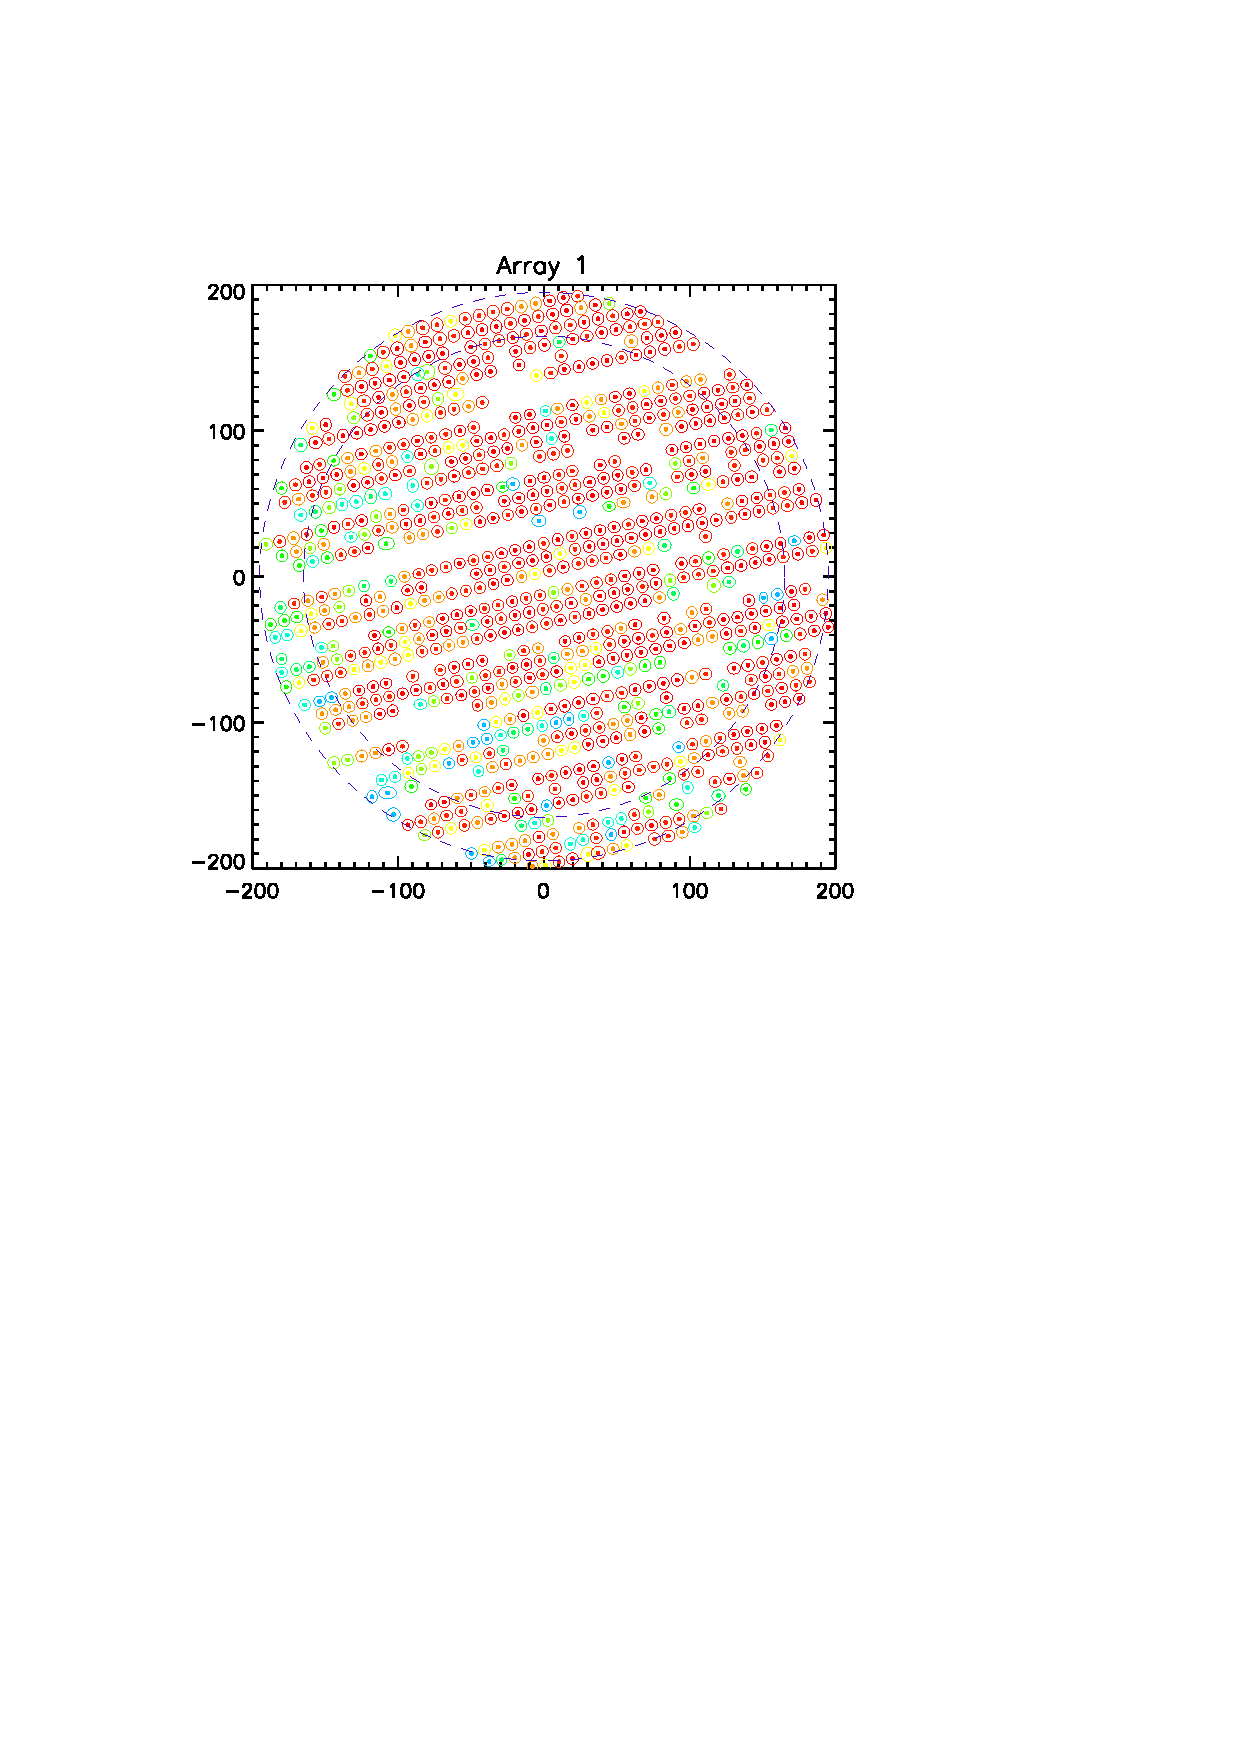
\includegraphics[trim=3cm 14cm 6cm 4cm, clip=true, width=0.32\linewidth]{Figures/A1_fwhm_color_count.pdf}
%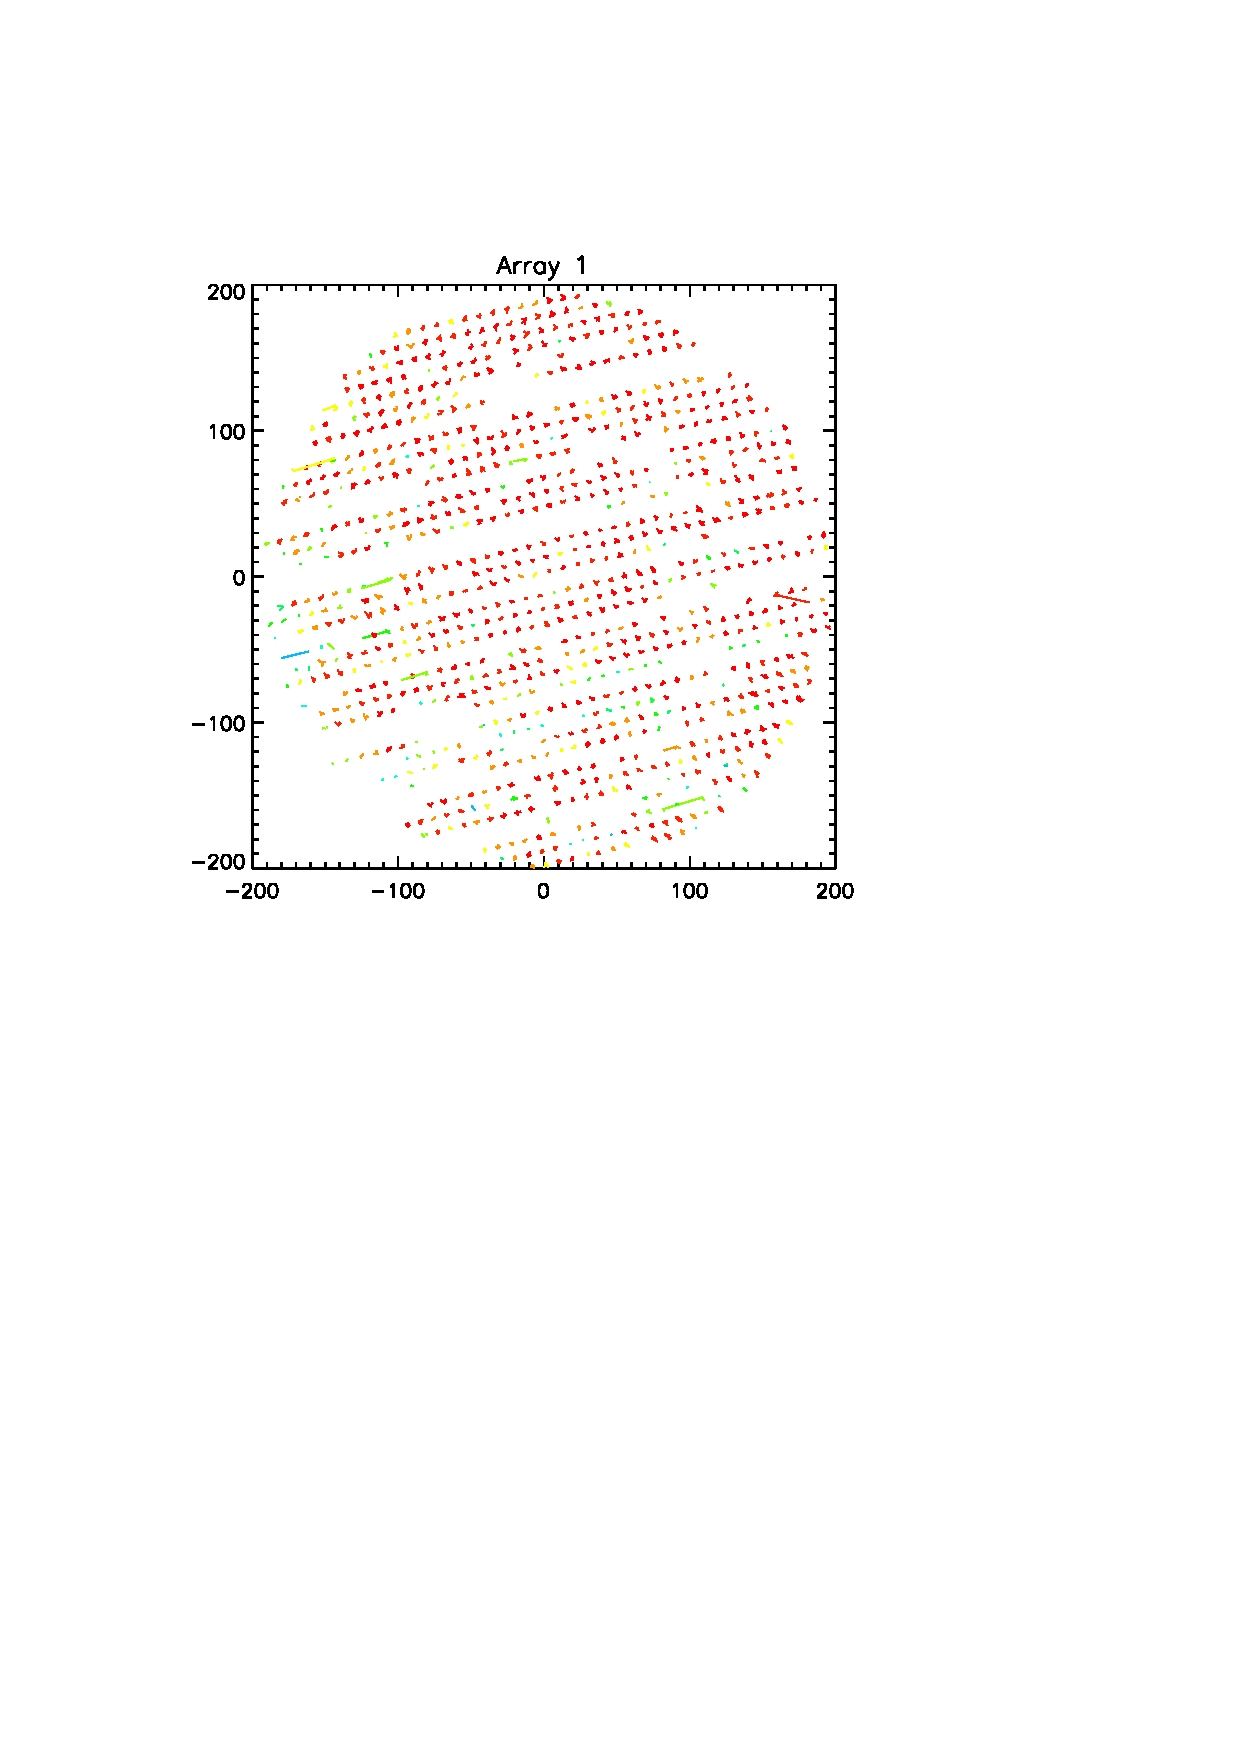
\includegraphics[trim=2cm 14cm 5cm 4cm, clip=true,width=0.45\linewidth]{Figures/A1_positions.pdf}
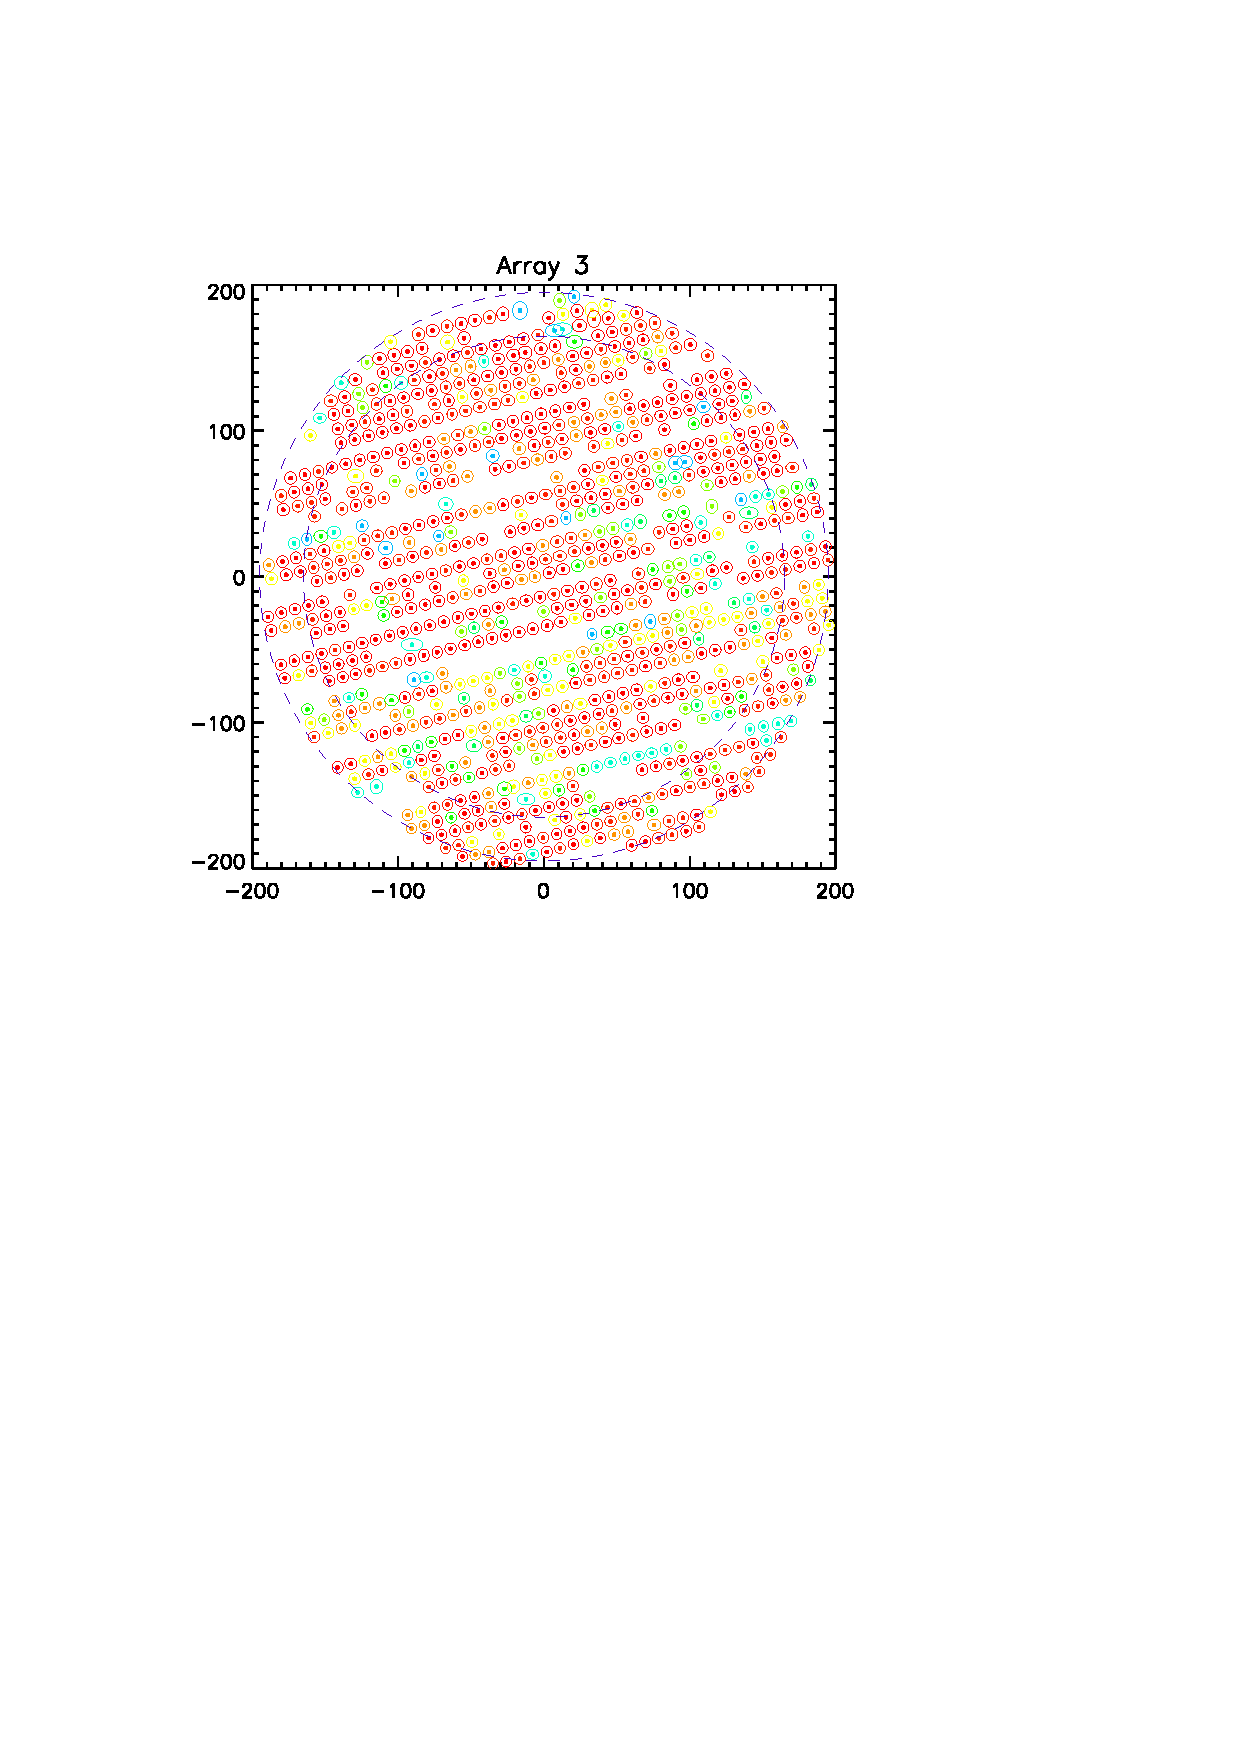
\includegraphics[trim=3cm 14cm 6cm 4cm, clip=true, width=0.32\linewidth]{Figures/A3_fwhm_color_count.pdf}
%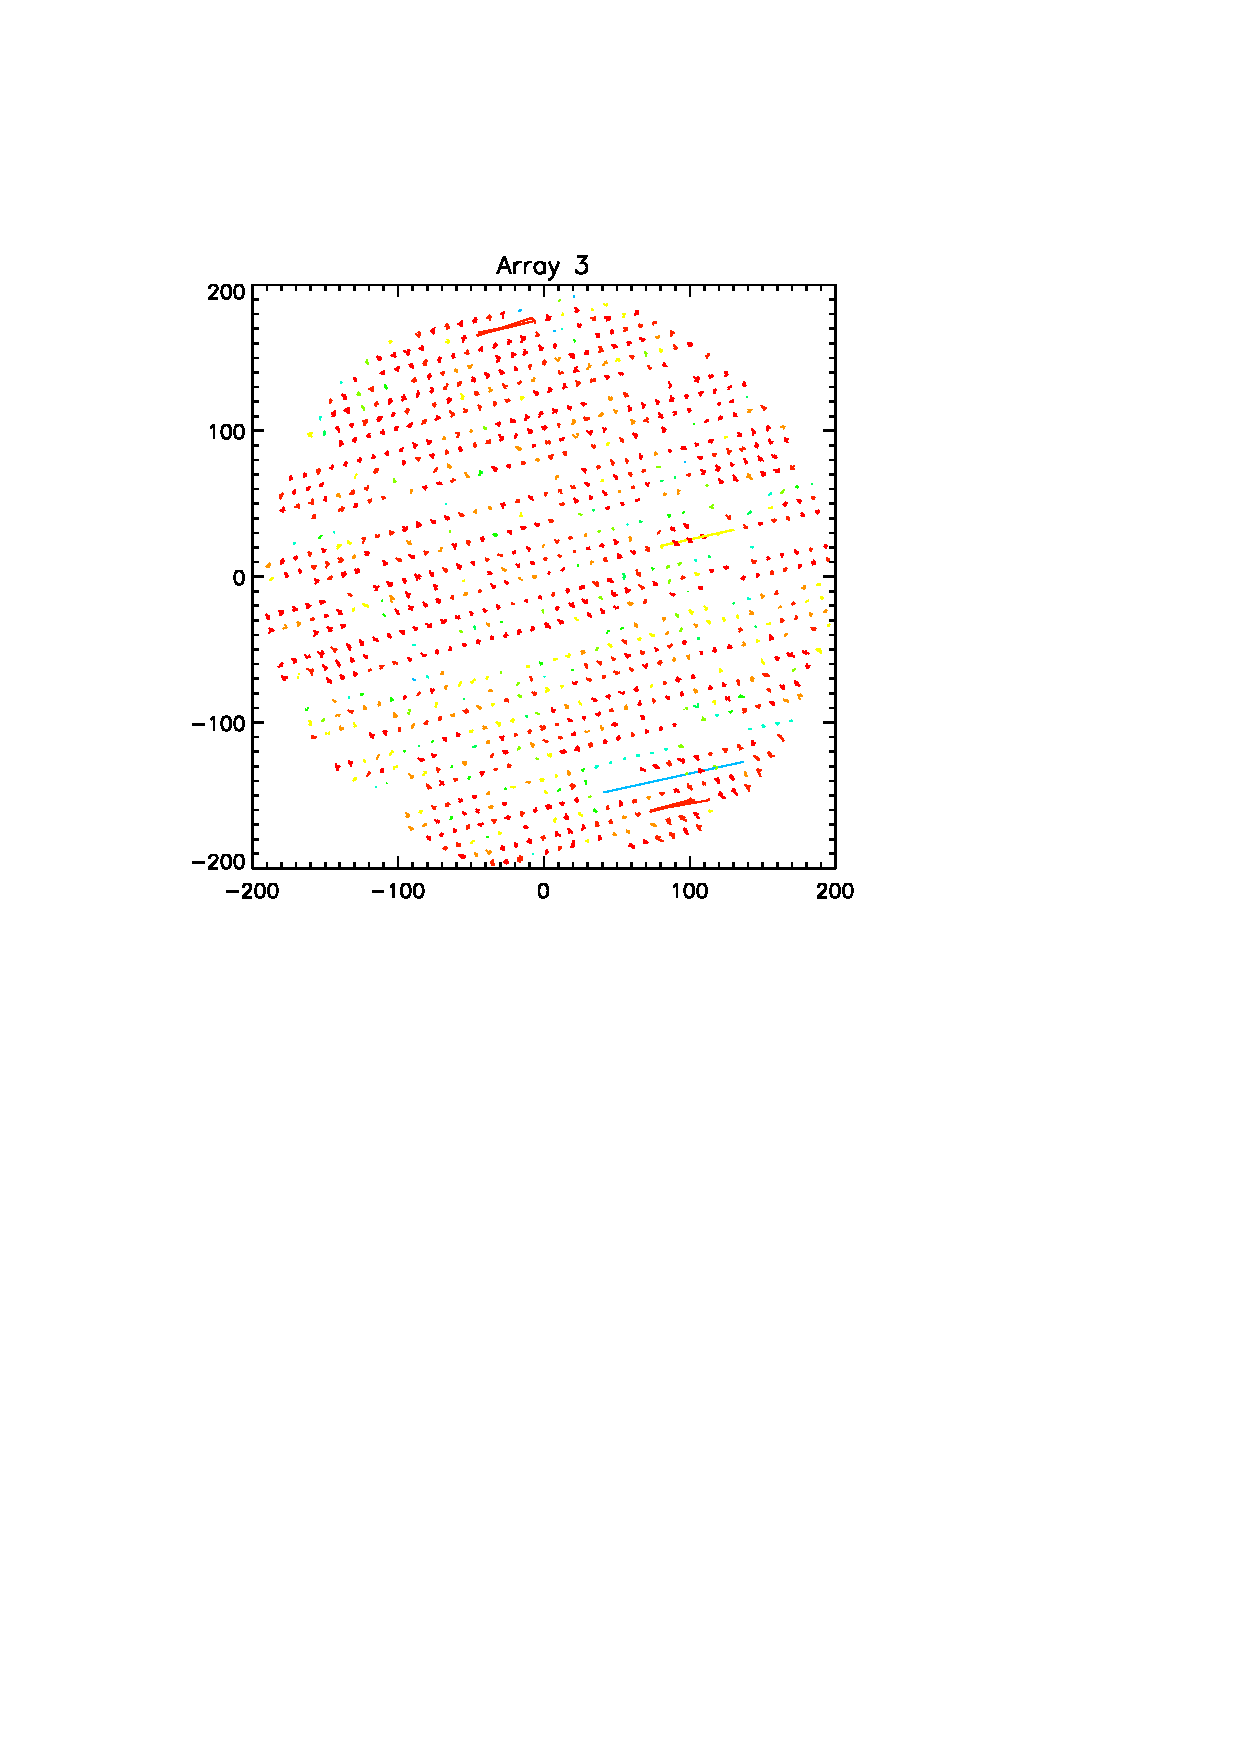
\includegraphics[trim=2cm 14cm 5cm 4cm, clip=true,width=0.45\linewidth]{Figures/A3_positions.pdf}
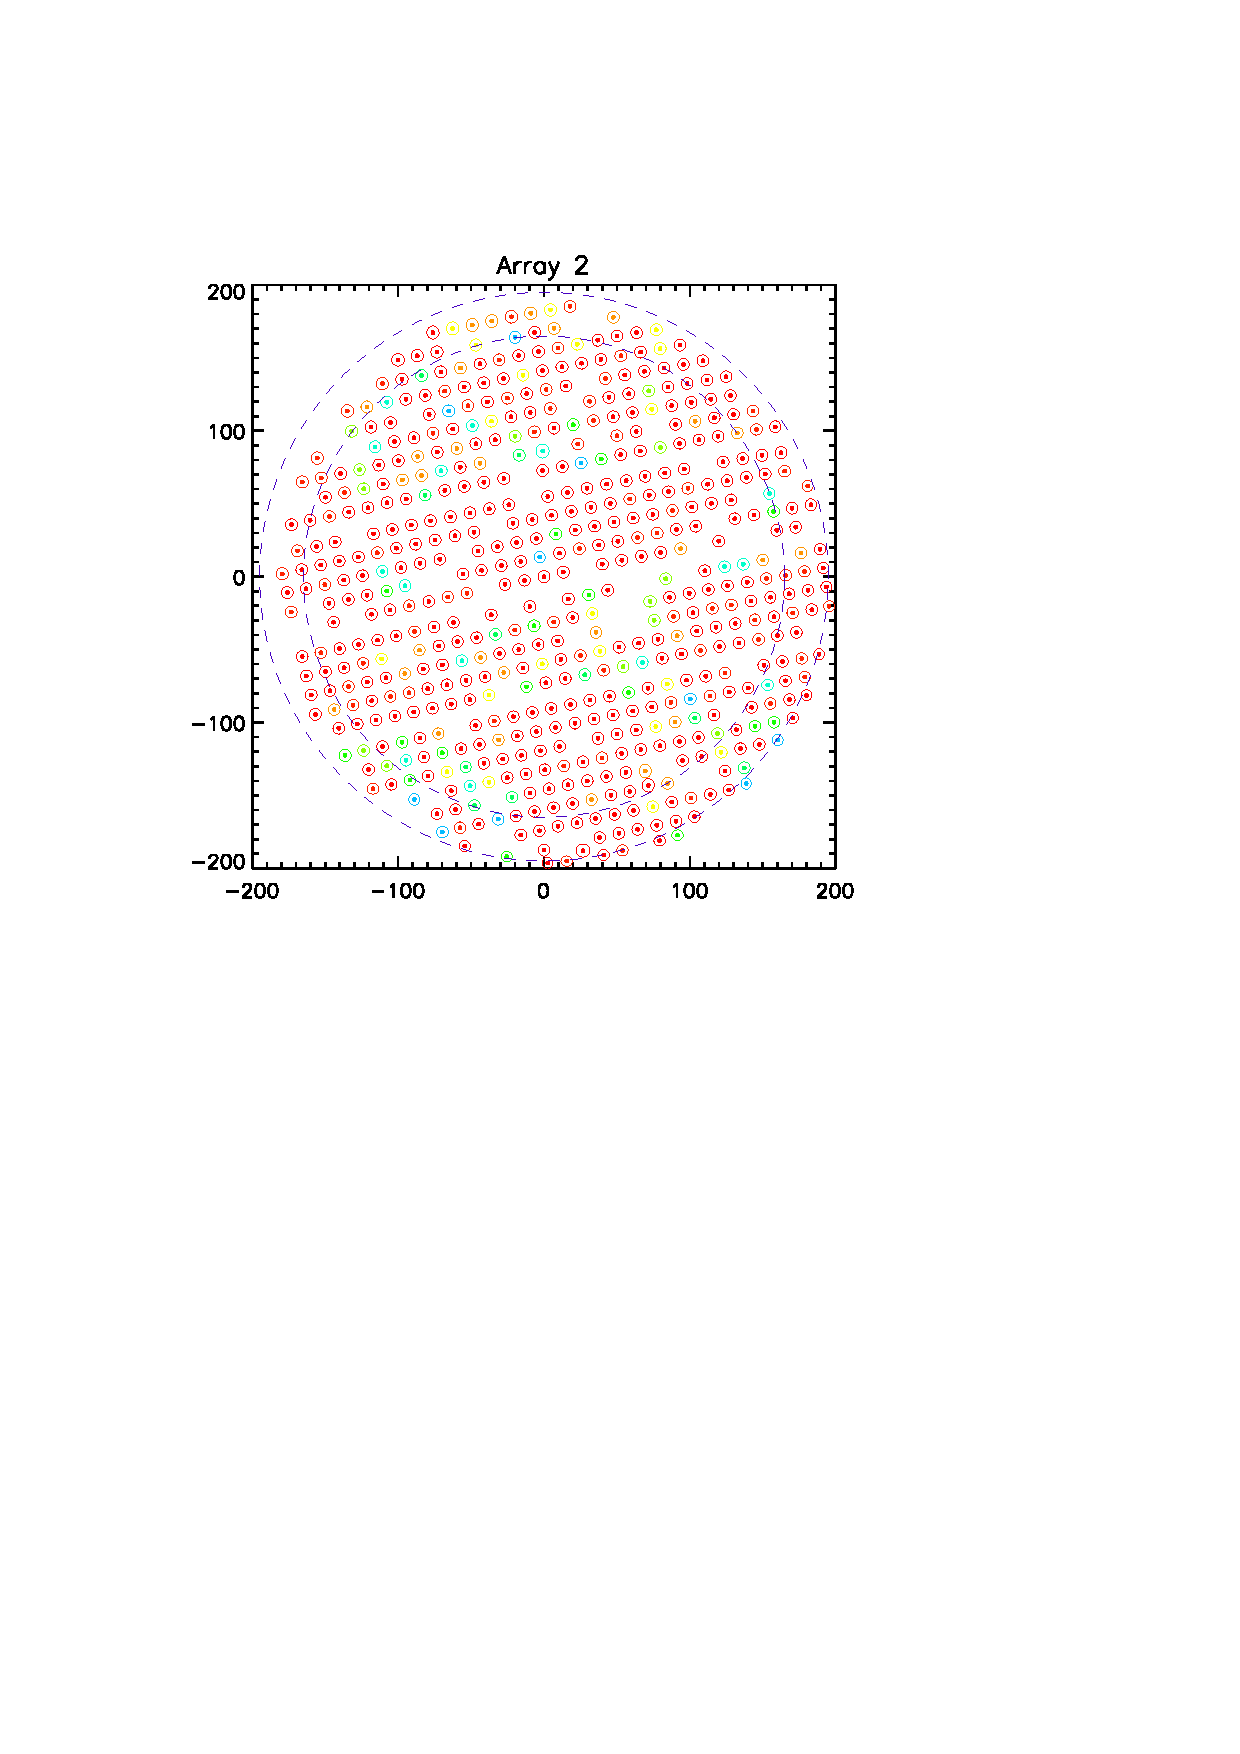
\includegraphics[trim=3cm 14cm 6cm 4cm, clip=true, width=0.32\linewidth]{Figures/A2_fwhm_color_count.pdf}
%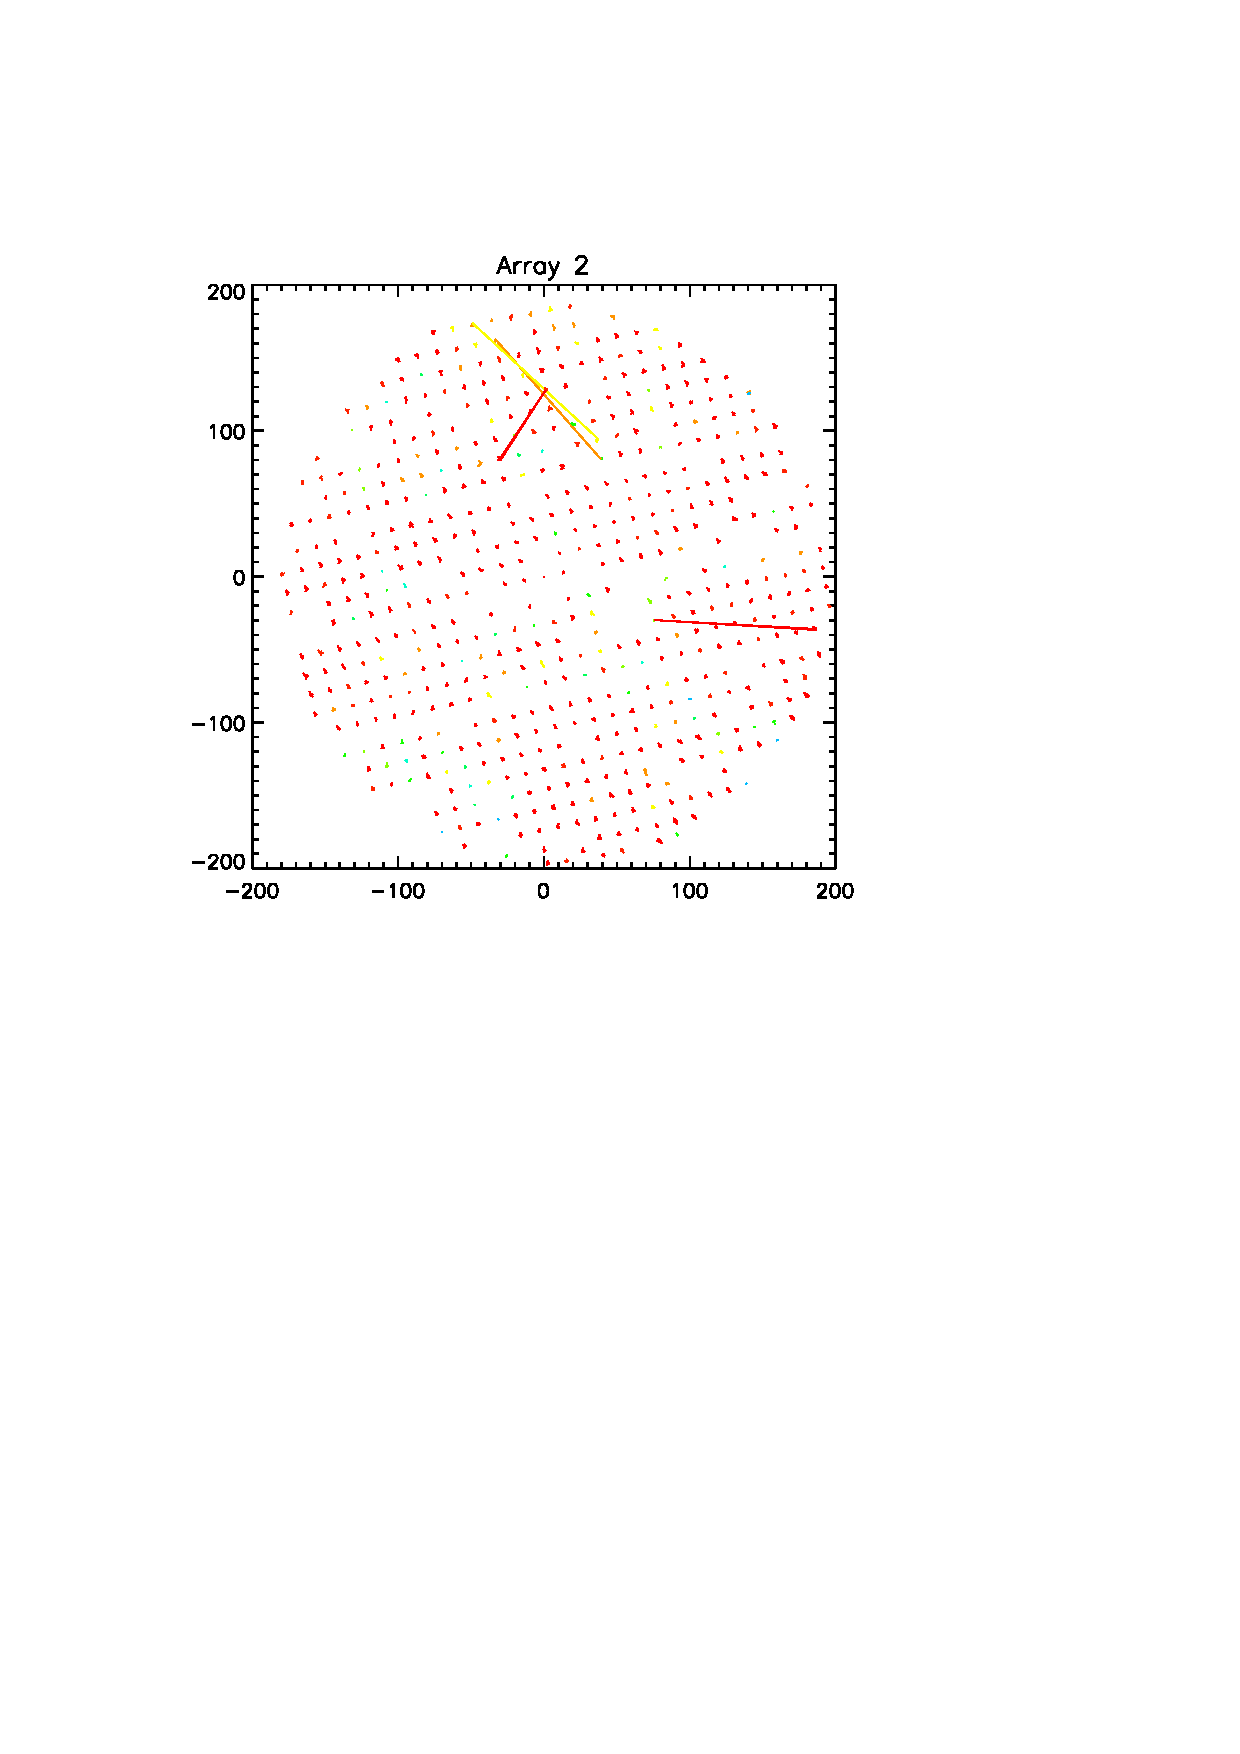
\includegraphics[trim=2cm 14cm 5cm 4cm, clip=true,width=0.45\linewidth]{Figures/A2_positions.pdf}
\caption[KID selection in the FOV]{Average detector positions
  for arrays A1, A3, and A2. The three plots show the detectors that
  met the quality criteria for at least two \bms\ during two technical
  campaigns. These consist of 952, 961, and 553 detectors for A1, A3
  and A2, respectively. The color
  indicates how many times a KID was identified as valid on a \bm,
  {\lp ranging from blue for the KIDs valid in at least two \bms, to red for the KIDs
  valid in all (ten) \bms.} 
  The inner and outer
  dash-line circles correspond to a FOV of 5.5\,arcmin and 6.5\,arcmin,
  respectively. Units are arcseconds.}
\label{fig:avg_fov_color}
\end{center}
\end{figure*}

\subsection{FOV grid distortion}
\label{se:grid_distortion}

We compare the reconstructed KID positions in the FOV to their design
positions in the array. We fit the 2D field translation and rotation that allow
matching the measured KID positions with the design positions using a 2D
polynomial mapping function. {\lp We find that a matching can be
obtained using a 2D polynome of degree one, that is using a linear
shift and a rotation only.} We call distortion cross-terms
between the two spatial coordinates in the polynomial fit.

The aim is twofold. First we obtain a detailed
characterisation of the real geometry of NIKA2 focal plane. Secondly,
{\lp this analysis is used for the KID
selection}, and the most deviant KIDs, whose measured position deviates
by more than $4''$ from the design position are discarded. 

We present the global results of the grid distortion
analysis using the KID positions given
by the focal plane geometry procedure, as described in
Sect.~\ref{se:fov_geometry}, applied to a \bm\ scan acquired
during the first scientific campaign (\aka\ N2R12). 
%Note that the
%selected KID numbers are low
%in this example as the scans were acquired during the daytime
%and suffers from temperature-induced instabilities (see
%Sect.~\ref{se:beam_variation}).
%We performed two tests. One test is based on using all the designed
%KIDs, while the second test relies on a KID selection applied in the
%FOV geometry obtained from the \bm\ scan. The KID selection, which
%consists in discarding the KIDs the most impacted by the cross-talk
%effect or the {\tt tuning} failures, is detailed in
%Sect.~\ref{se:avg_kidpar}.
The initial
number of KID considered in this analysis results from
a first KID selection, which consists in discarding the KIDs that are the most
impacted by the cross-talk effect or the {\tt tuning} failures,
applied in the FOV geometry obtained from the \bm\ scan. More details
on the KID selection are given in the next section. %Sect.~\ref{se:avg_kidpar}.
The results are gathered in Table~\ref{ta:gridmatch}.

\begin{table}[!htbp]
  \caption[Field-of-view deformations]{Field-of-view
  deformation. Example of mapping of the observed KID positions in the
  sky to their mechanically designed positions. The initial table of
  selected KIDs is given by the focal plane geometry procedure, as
  described in Sect.~\ref{se:fov_geometry}, applied to a \bm\ scan
  acquired during the N2R12 campaign. %Note that the selected KID numbers are particularly
    %low in this example, as the scans were observed during the daytime
    %and suffer from temperature-induced instabilities (see
    %Sect.~\ref{se:beam_variation}). Even in this pessimistic case,
    More than 90\% of the detectors are within less than 5 arcseconds
    of their expected position.}
  \label{ta:gridmatch}
  \centering
  \begin{tabular}{r|c|c|c}
    \hline
    \hline
    Characteristic &  Array 1  &	Array 3   &	Array 2  \\
    \hline
    %\small{$\lambda$ [mm]}  &  1.25     &      1.25      & 2.05   \\
    \small{$\lambda$ [mm]}  &  1.15     &      1.15      & 2.0  \\ 
    \small{Design detectors} & 1140  &  1140 & 616  \\
    %\small{Well-placed KID}                  &  864  &  808  & 488  \\
    \small{Selected KID}\tablefootmark{a}    &  866  &  808  & 488  \\
    \small{Well-placed KID}\tablefootmark{b}          &  864  &  808  & 488  \\
    %\small{Ratio [\%]}\tablefootmark{b}      &  76   &  71   & 79   \\
    %&673/736  &	734/758   &    437/444   & \small{Well-placed KIDs (WPK)/Found KIDs (FK)} \\
    %&91/59 	 &      96/64 	  &    98/71 	 & \small{Ratio [\%] of WPK/FK and WPK/TDK} \\
    \small{Median deviation\tablefootmark{c}  [arcsec]}    & 1.01    &     0.95   &    0.75  \\
    \small{Mean distortion\tablefootmark{d} [arcsec]}                       & 1.09    &     1.01   &    0.84  \\
    \small{Array center\tablefootmark{e} [arcsec]}  & (1.9, -5.1) & (2.3, -6.2) &  (9.6, -7.8) \\
    \small{Scaling\tablefootmark{f} [arcsec/mm]}   &  4.9     &	4.9      &    4.9 \\
    %& \small{Plate scaling [arcsec/mm] in the Design x and y (averaged)} \\
    \small{Rotation angle\tablefootmark{g} [degree]} & 77.3     &	76.3      &    78.2  \\
    %\small{FOV [arcmin] (Total KIDs)}                      & 6.6      &	6.6       &    6.6   \\
    \small{Grid step\tablefootmark{h} [arcsec, mm] }     & 9.8, 2.00 &	9.7, 2.00  &    13.3, 2.75 \\
    % Old values, rechecked (difference comes from lambda and D)
    %   1.24  &	1.22  &	0.97  &	Distance between near detectors with $30\,\rm{m}$ diameter aperture [in $\lambda$/D] \\
    % here new values checked FXD 30 Nov 2018 1.11 1.10 0.87
    \small{Grid step\tablefootmark{i} [$\lambda$/D] } & 1.11     &	1.10      &	0.87  \\
    %\new{with $27\,\rm{m}$ effective diameter aperture} [in $\lambda$/D]} \\
    \small{Modeled grid step\tablefootmark{j} [$\lambda$/D]}  & 1.09     &      1.09      & 0.93    \\
    \hline
  \end{tabular}
  \tablefoot{ \\
    %\tablefoottext{a}{Initial number of KIDs given in a FOV geometry
    %  for the N2R9 campaign (pessimistic case)}
    \tablefoottext{a}{Initial number of KIDs selected in a FOV geometry using a \bm\ scan of the N2R12 campaign;}
    %\tablefoottext{b}{Ratio of the well-placed KID to the designed KID numbers}
    \tablefoottext{b}{{\lp Number of KIDs whose the best-fit sky position is at less than 4'' from
the expected position;}}       
    \tablefoottext{c}{{\lp Median angular offset [arcsec] between the expected and measured sky position of the KIDs;}}
    \tablefoottext{d}{{\lp Average best-fit cross term of the polynomial model across the FOV [arcsec];}}
    \tablefoottext{e}{Array center in Nasmyth coordinates;}
    \tablefoottext{f}{Averaged scaling between measured {\lp KID position
  grid} and the designed one;}
    \tablefoottext{g}{Rotation from the design to Nasmyth coordinates;}
    \tablefoottext{h}{Center-to-center distance between neighbour detectors;}
    \tablefoottext{i}{Center-to-center distance between neighbour detectors using the
  reference frequencies ($260\,\rm{GHz}$ and $150\,\rm{GHz}$) and a
  27\,m {\lp entrance pupil diameter} (see Sect.~\ref{se:instru_optics});}
    \tablefoottext{j}{Center-to-center distance between neighbour detectors modeled using ZEMAX simulation.}
  }
\end{table}

Most of the selected KID are also well-placed, that is at less than 4'' from
their expected position. Moreover, on average the position of each
detector is known to about one arcsecond. We find
that Array 1 has some of the most deviant detectors (above 4''
from their expected position). These detectors are excluded from
further analysis. The two 1\,mm arrays have almost
the same center but this center differs by $7''$ and $2''$ in the two Nasmyth
coordinates, respectively, from the 2\,mm array center. This has no impact on the
pointing nor the focus settings. {\lp The center-to-center distance between
contiguous detectors, referred to as grid step, has been estimated in
$mm$ and arcseconds. The ratio of the grid step in mm to
the grid step in arcseconds gives compatible effective focal lengths
of about $42.4\pm0.3\,\rm{m}$ at both observing wavelengths.} The sampling is above $\lambda/D$ at
1\,mm, assuming a 27\,m effective diameter aperture. Note that
the rotation angle between the array and the Nasmyth
coordinates was designed as $76.2^{\rm{o}}$, less than two degrees from
what is observed.


These results have been compared to expectations obtained using ZEMAX
simulation. 
%The grid diagram generated using ZEMAX provides us with
%the maximum dispersion in the field defined by
%
%\begin{equation}
%P = \frac{\sqrt{(x_p - x_r)^2 + (y_p - y_r)^2}}{\sqrt{x_p^2 + y_p^2}},
%\end{equation}
%
%where $(x_p, y_p)$ and $(x_r, y_r)$ are respectivelly the predicted
%and real coordinates on the image surface relative to the reference
%field position image location (see page 170 of the ZEMAX manual, 2007).
%The predicted coordinates for the whole field are obtained using a
%linear interpolation of a small area in the field central part,
%whereas the real coordinates are calculated by ray tracing through the
%optical system.
%
%\begin{figure}[ht] 
%\begin{center}
%  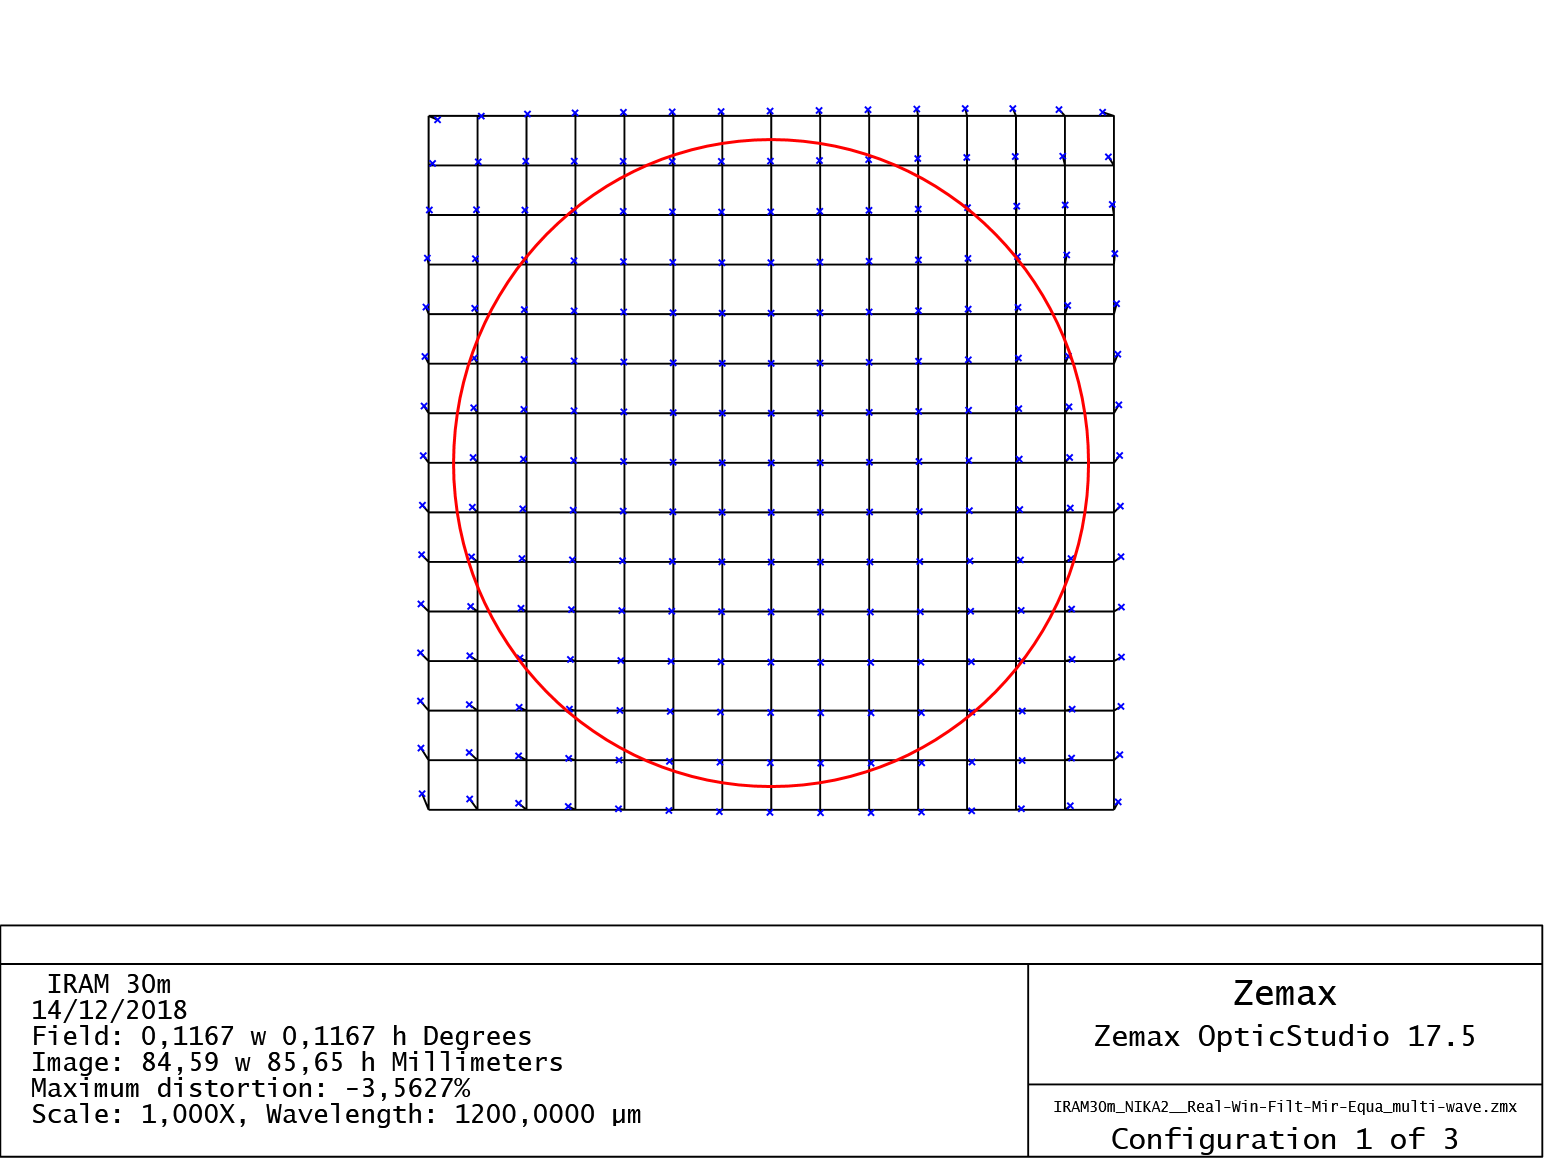
\includegraphics[width=0.9\textwidth]{Figures/NIKA2_Grid-distortion.png}
%  \caption[Simulated FOV grid]{NIKA2 grid diagram simulated using
%    ZEMAX. \new{The step of the grid is of 30 arcsec and the side width
%      of the black square is of seven arcmin. The red circle corresponds to the 
%      $6.5\,\rm{arcmin}$ diameter FOV. Blue crosses show the grid
%      distorsions in az-el coordinates and in the case of an observing
%      elevation of $14^o$. These grid distorsions depends on the
%      telescope elevation, whereas in the image plane (the plane of the
%      KID arrays) the distorsions are invariant. This allows for
%      concluding that the grid distorsions are caused by the optical
%      elements located between M4 and the dichroic plate.} 
%  }
% \label{fig:fov_grid_distortion_zemax}
%\end{center}
%\end{figure}
%Figure \ref{fig:fov_grid_distortion_zemax} shows the ZEMAX grid diagram for
%NIKA2 simulated optic system.
%
We generated a grid diagram for the NIKA2 optical system and found a maximum
grid distortion of $2.7\%$ in the $6.5'$ FOV. We notice that the
strongest distortion appear in the upper right corner of the Nasmyth plan, which is
also the area of the largest defocus w.r.t. to the center (see Appendix~\ref{ap:focus_surfaces}).
An expected distortion of $2.7\%$ is at most a 5'' shift from the
center to the outside of the array. The quoted distortions between the
measured and design positions are well within the expected
maximum distortions from the NIKA2 optics.

%Auxillary information on this work can be found in this wiki post\footnote{\tiny
%  {\tt http$://$www.iram.fr$/$wiki$/$nika2$/$index.php$/$April$\_$19,$\_$2017,$\_$FXD,$\_$KID$\_$position$\_$mapping$\_$and$\_$Field$\_$distortion$\_$for$\_$Run9}}.
% FXD: this would need to be more ascertained. Lack of time to go further.


\subsection{KID selection and average geometry}
\label{se:avg_kidpar}

In order to identify the most stable KIDs, we compare the KID parameters
obtained using the FOV reconstruction procedure, as described in
Sect.~\ref{se:fov_geometry}, with several \bms. In the following, we
show results as obtained using {\lp ten} \bms\ acquired during two
technical observation campaigns in 2017.
%7 from Run10, two from Run9 and one from Run8.
For each KID we compute the average position on the focal plane and
the average FWHM. 
As discussed in Sect.~\ref{se:fov_geometry}, we perform a KID
selection while analysis a \bms. A few KIDs have very close resonance
frequencies and can be misidentified on some scans. A few others must
also be discarded because they appear identical
numerically due to the fact that a same (noisy) KID can sometimes be
associated to two different frequency tones in the acquisition system.
These KIDs are flagged out (less than 1\% of the design KIDs).
{\lp We count the times that a KID has been kept in
the KID selection and that it has been found at a position agreeing
with its median position within 4''.}
We define the {\emph valid} KIDs as the KIDs that met the selection
criteria in about {\lp $20\%$} of the FOV geometries (in two \bm\
analysis out of ten).

In Fig.~\ref{fig:avg_fov_color} we show the average focal plane
reconstruction. The colors, from blue to red,
represent the number of times that the KID has been retained after
KID selection. The eight feed lines for each of the two
$1\,\rm{mm}$ arrays {\lp can also be traced out in several ways} in this
figure. First, slightly larger spaces are seen between KID rows
connected to different feed lines than between KID rows of the same
feed line. Second, KIDs at the end of a feed line are less often valid
than the others
(see e.g. the FOV of Array 3). As the tone frequencies
increase with the KID position in the feedline, some KIDs are
sometimes missing because their frequency lays above the maximum tone
frequency authorized by the readout electronics. That explains the
linear holes in the middle of the $1\,\rm{mm}$ arrays. For A1, this
end-of-feedline effect is mixed with the effect of the KID gain
variation across the FOV, which mainly affects the lower left third of
the array, as discussed in Sect.~\ref{se:flat_field}.

For A1, A3 and A2, respectively, we found 952, 961, and 553 valid KIDs
 (selected at least twice). From this, we deduce the fraction of
valid detectors over the design ones, as given in Table~\ref{tab:number_of_kids}.

%% \begin{figure}[htp]
%% \begin{center}
%% 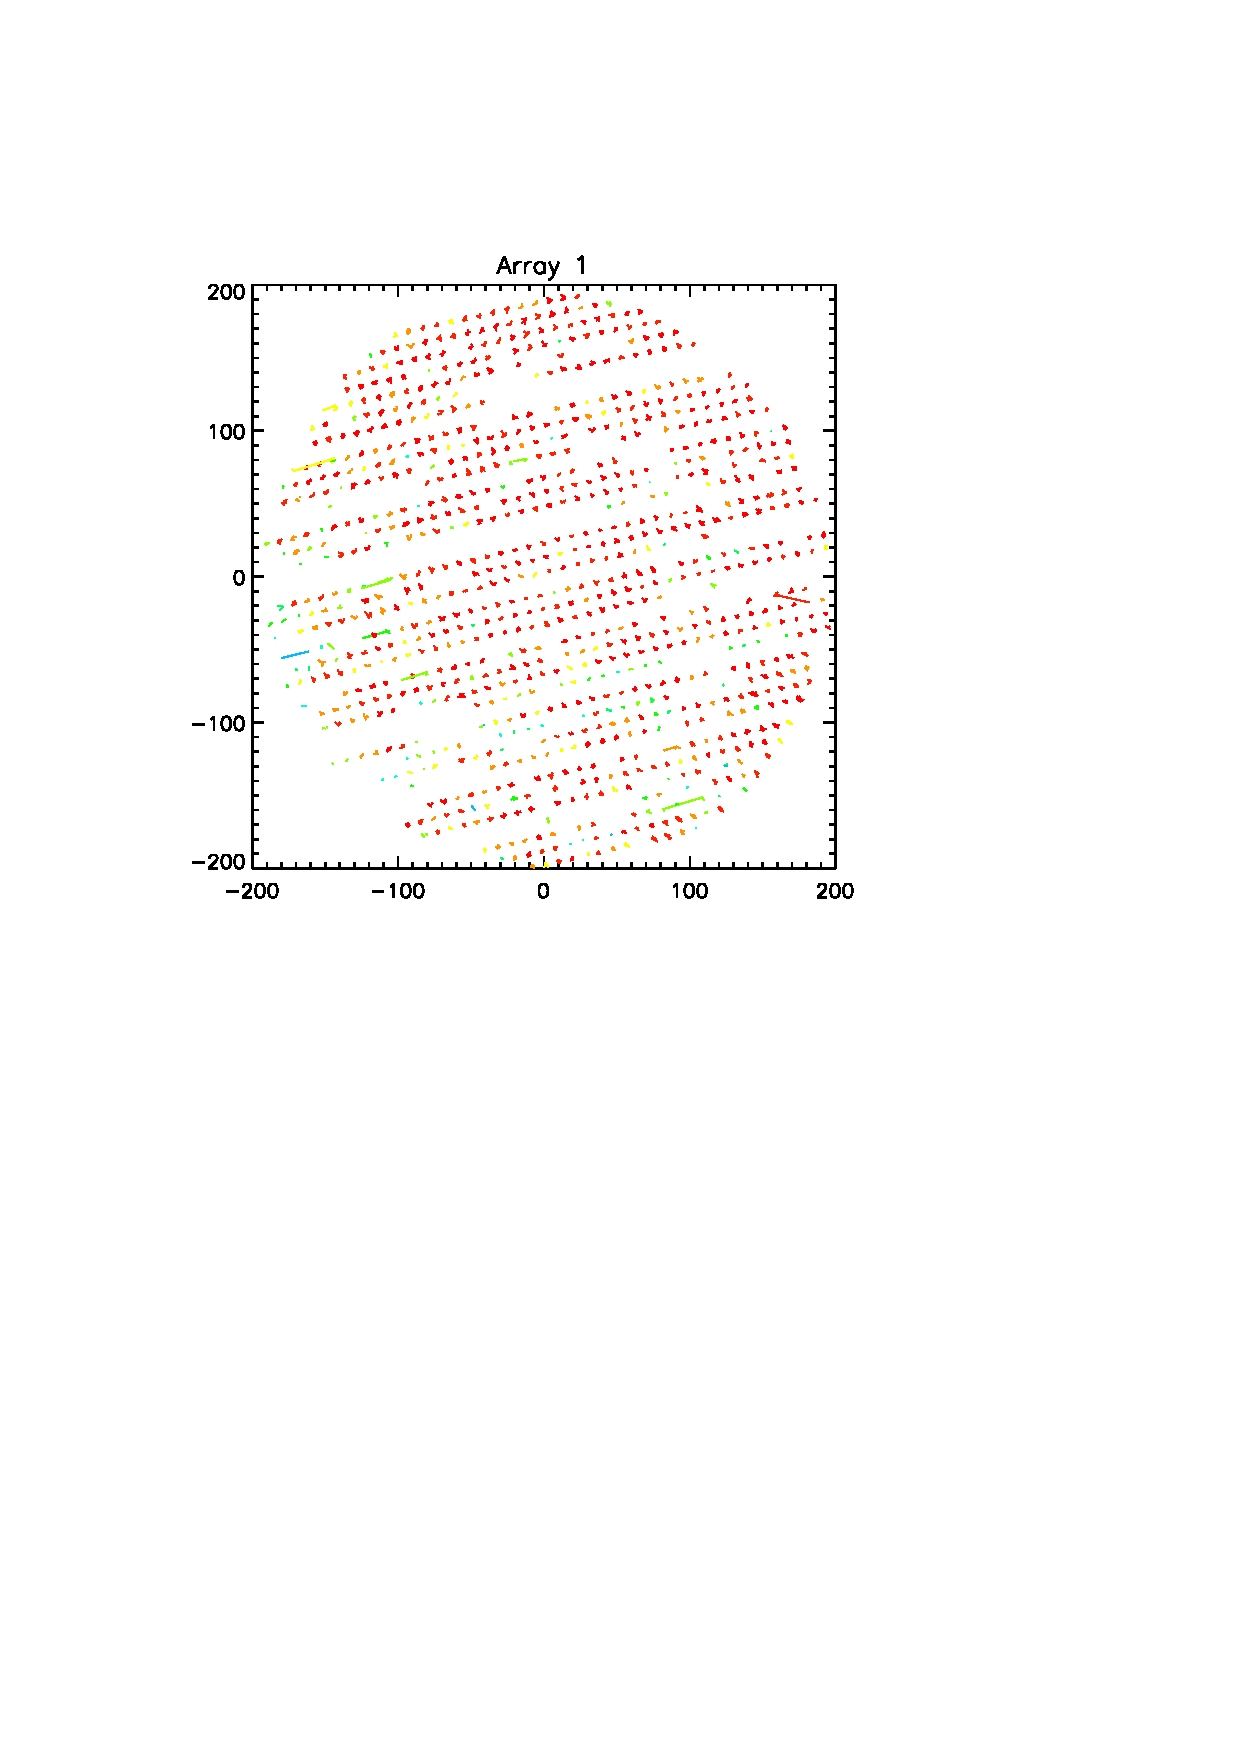
\includegraphics[trim=2cm 14cm 5cm 4cm, clip=true,width=0.55\linewidth]{Figures/A1_positions.pdf}
%% 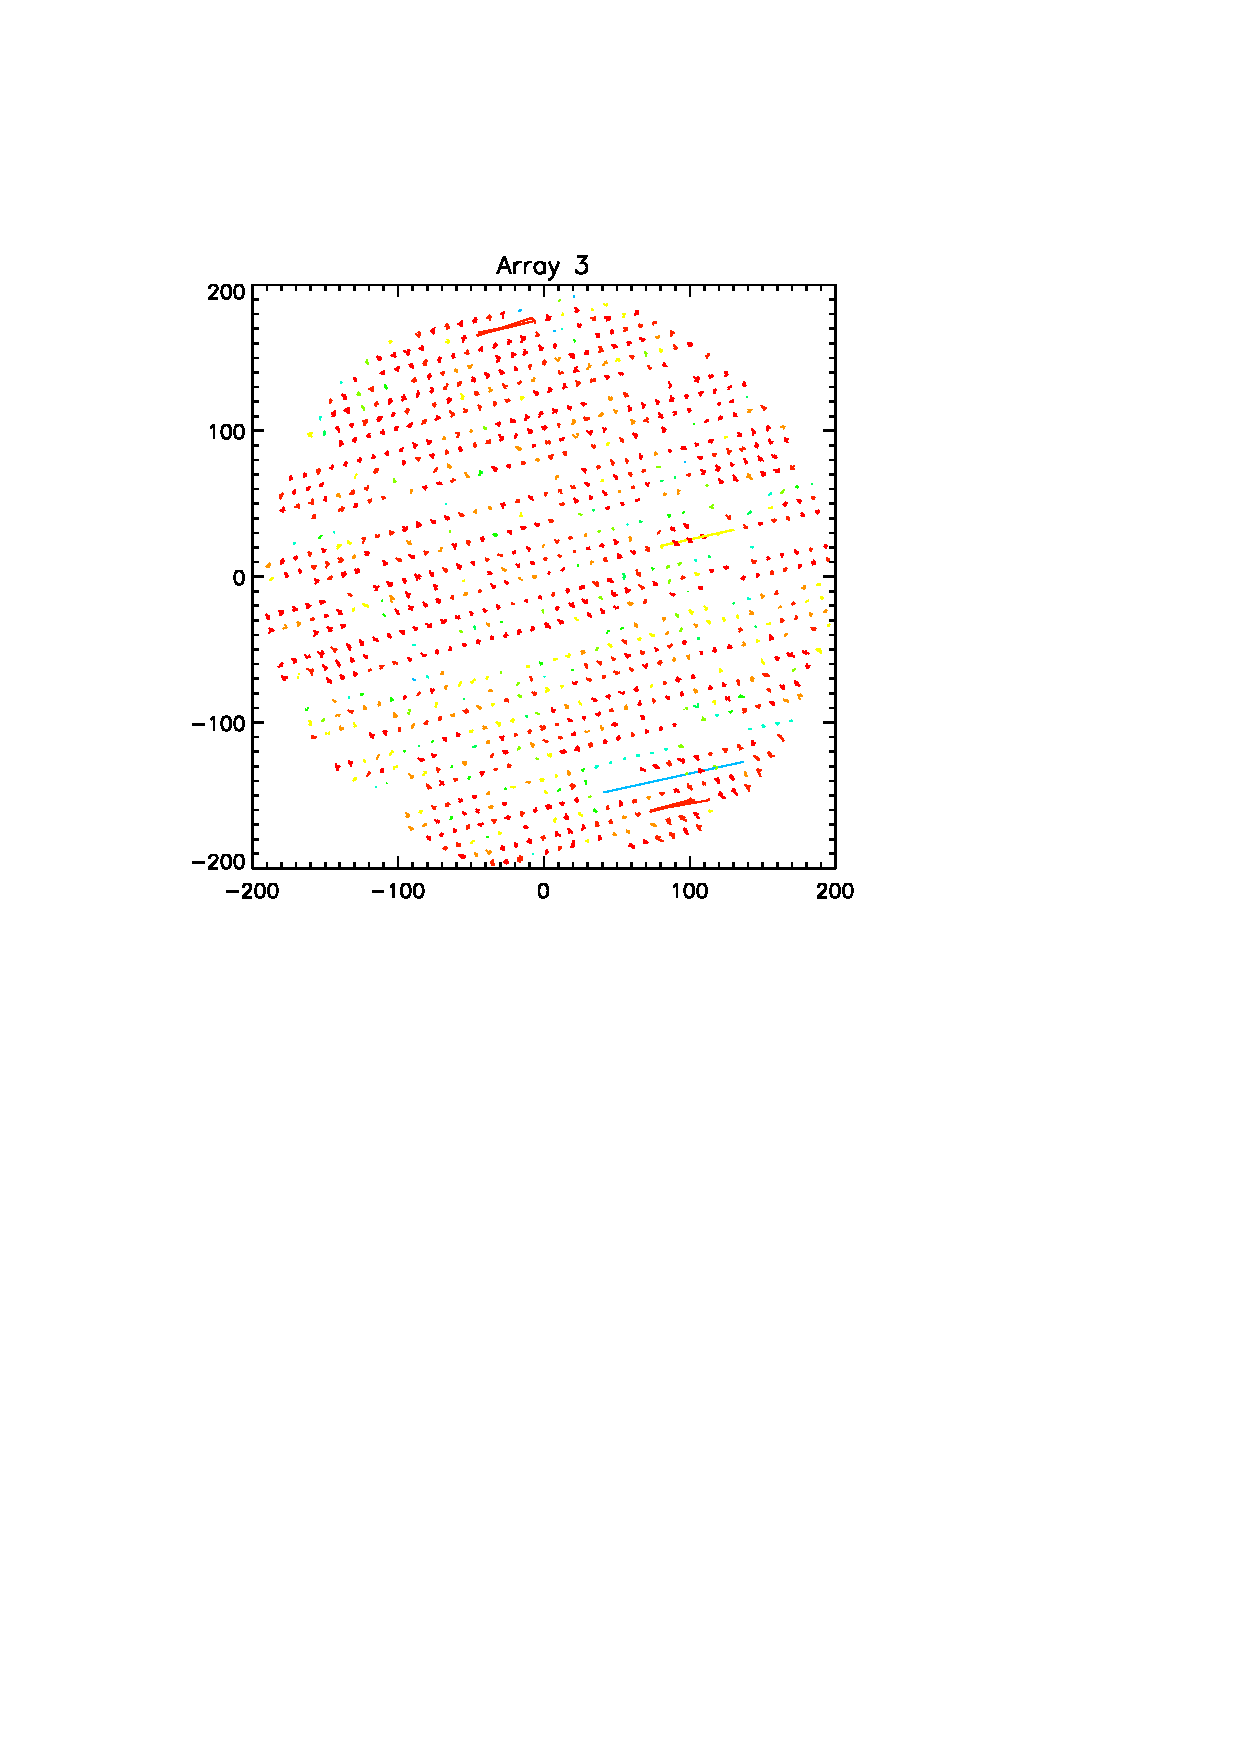
\includegraphics[trim=2cm 14cm 5cm 4cm, clip=true,width=0.55\linewidth]{Figures/A3_positions.pdf}
%% 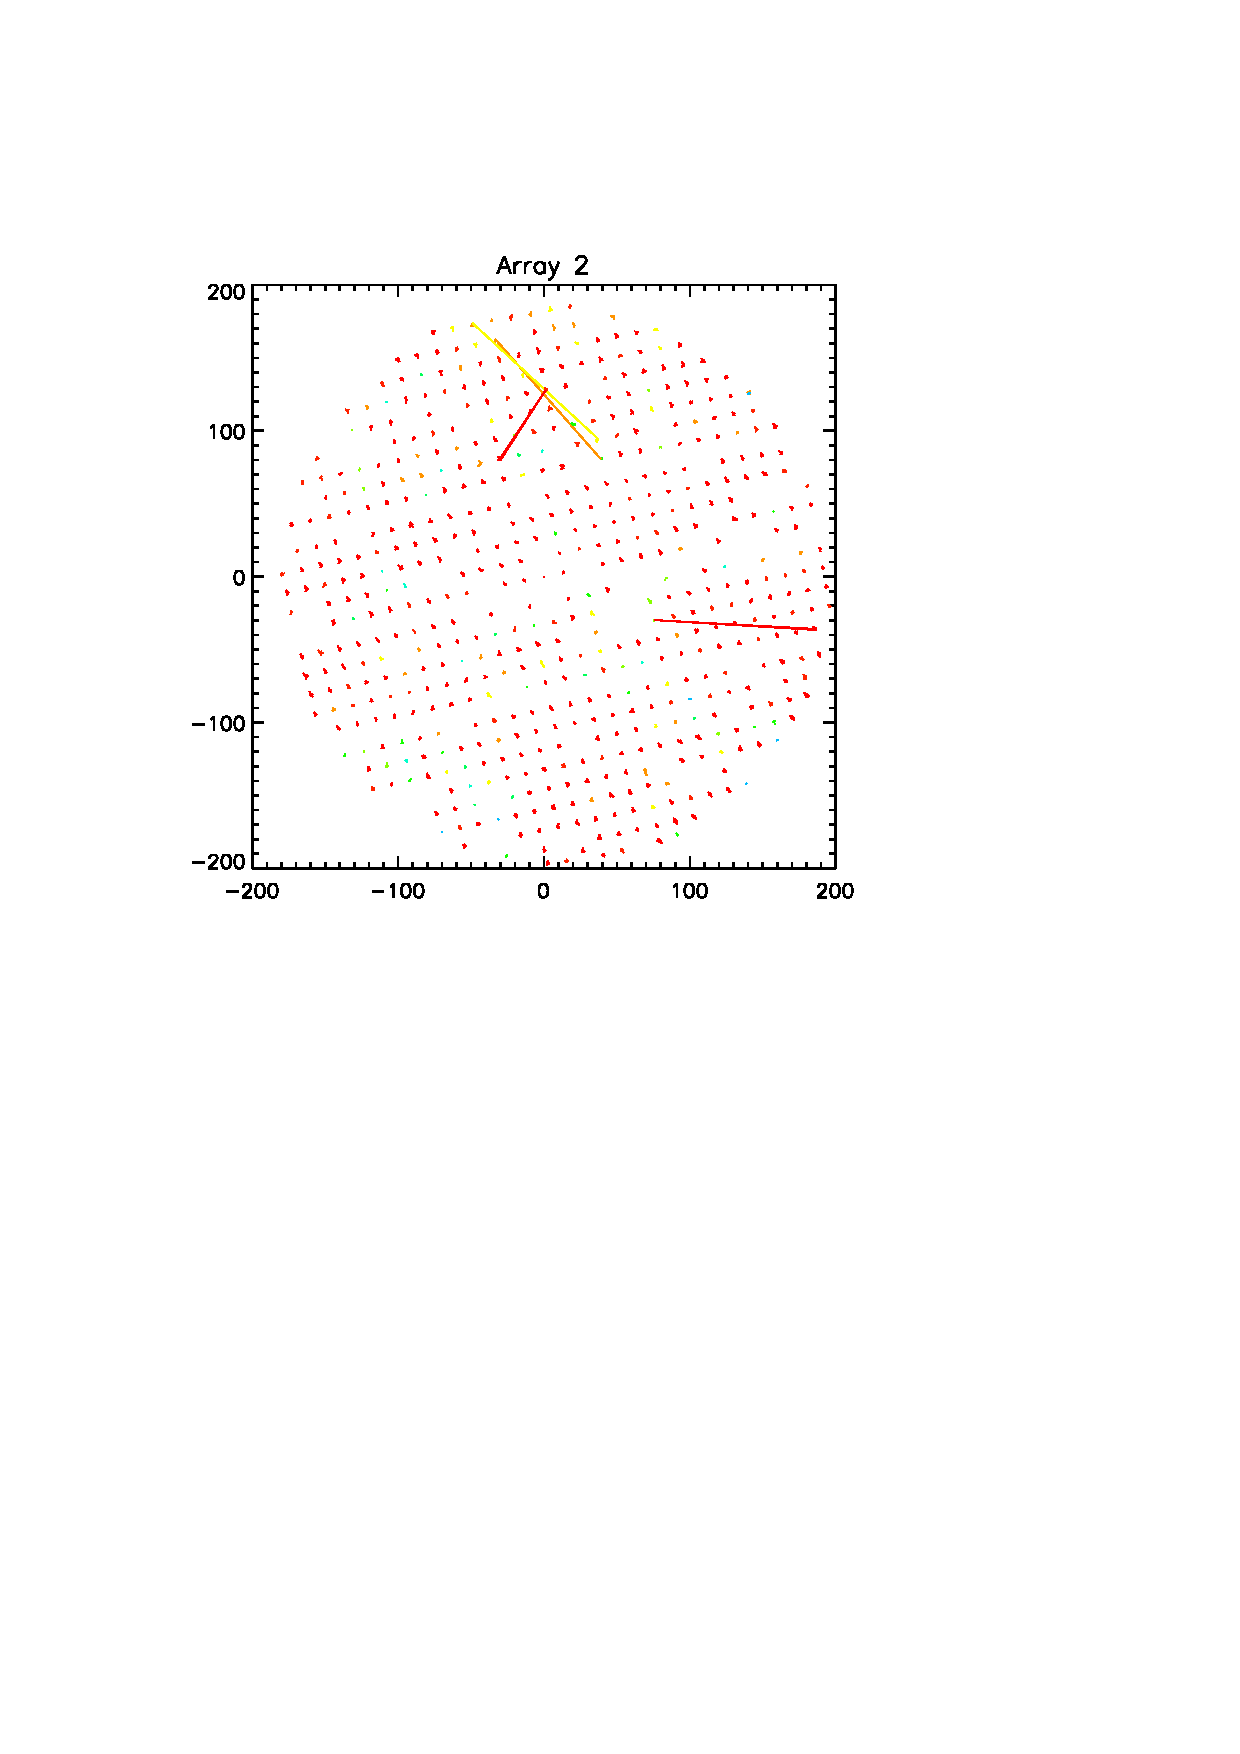
\includegraphics[trim=2cm 14cm 5cm 4cm, clip=true,width=0.55\linewidth]{Figures/A2_positions.pdf}
%% \caption[Stability of KID positions in the field-of-view]{For the valid
%%   detectors, we show the positions of each pixel, as obtained from each beam
%%   map. Some of them are not found at the same position for all the \bms.
%% Units are arcseconds. \todo{{\bf FM : color code : same as on the 1st
%%       maps of validity}}}
%% \label{fig:jumping_kids}
%% \end{center}
%% \end{figure}

%\begin{figure}[htp]
%\begin{center}
%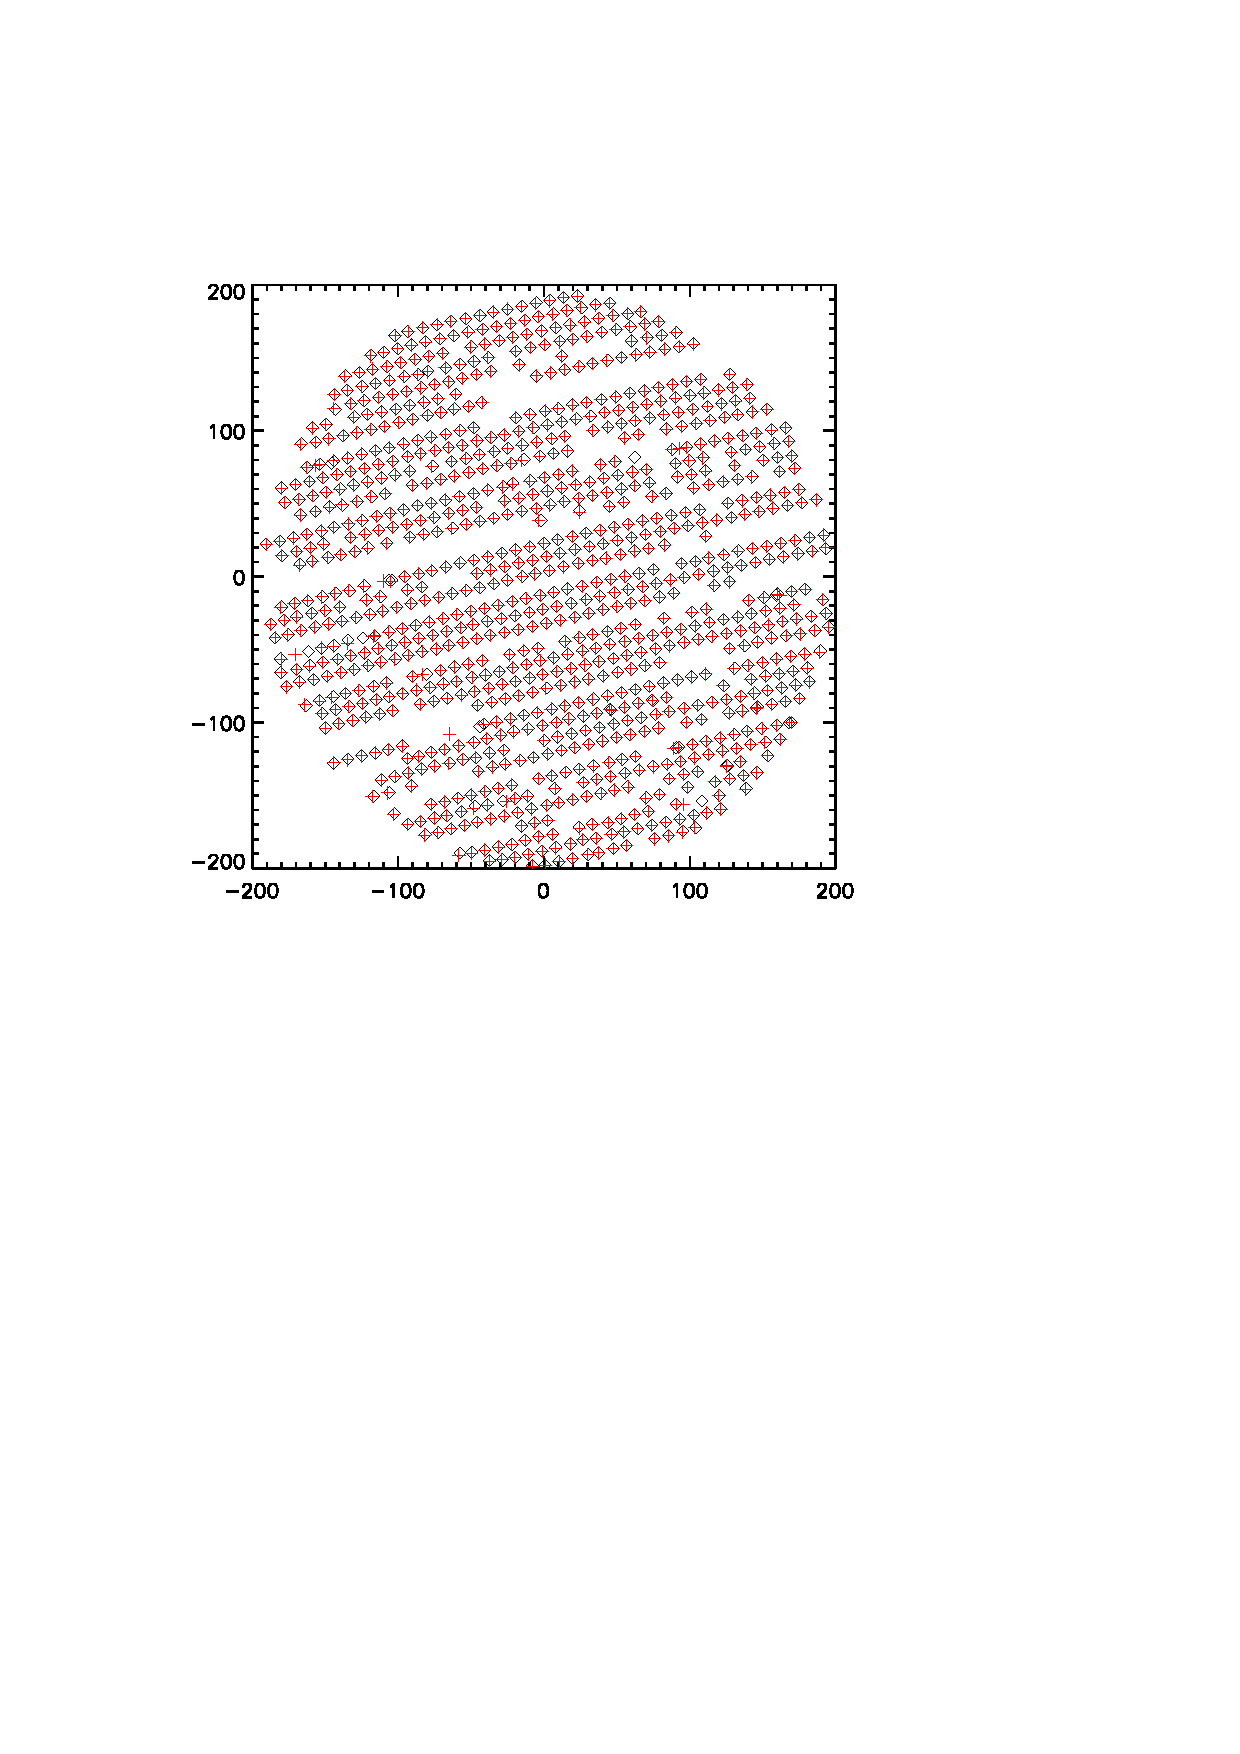
\includegraphics[trim=2cm 14cm 5cm 4cm, clip=true,width=0.55\linewidth]{Figures/A1_test_positions.pdf}
%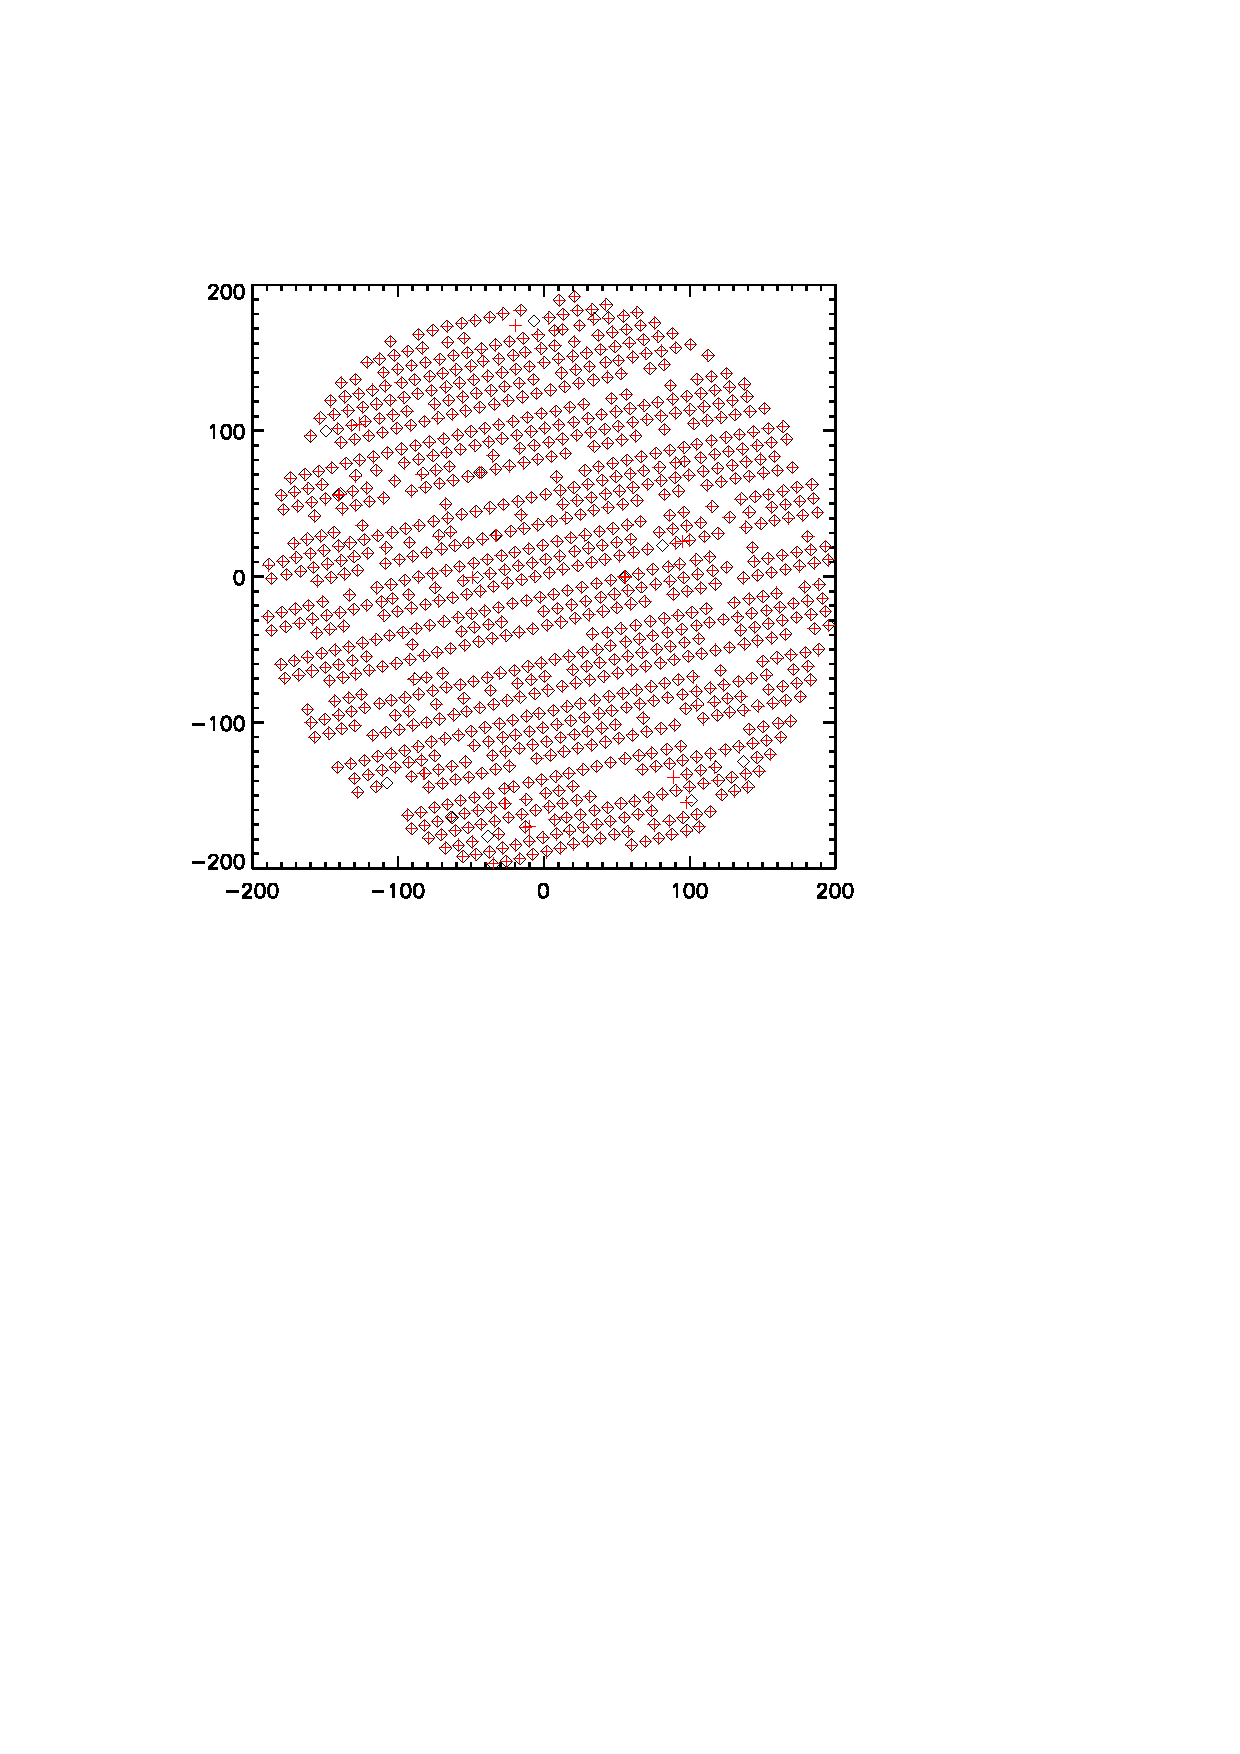
\includegraphics[trim=2cm 14cm 5cm 4cm, clip=true,width=0.55\linewidth]{Figures/A3_test_positions.pdf}
%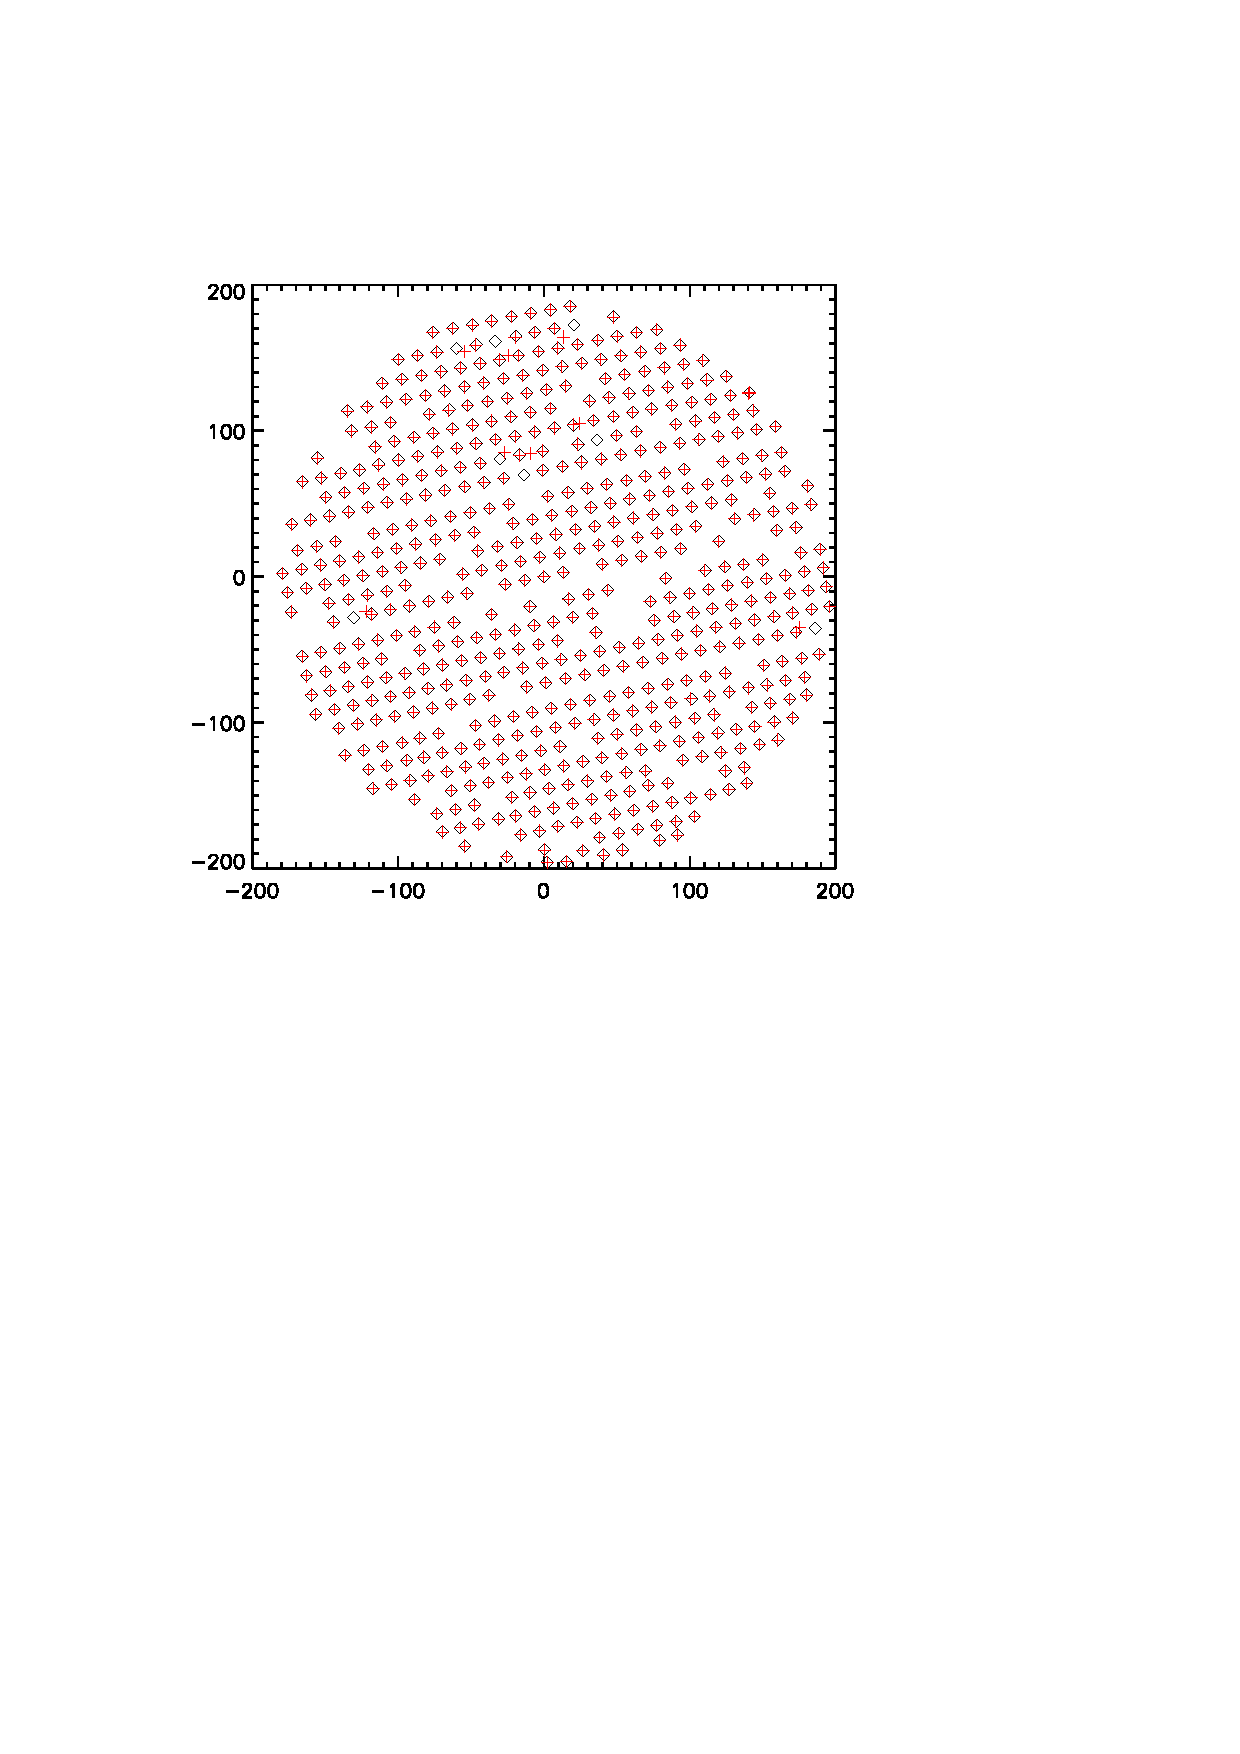
\includegraphics[trim=2cm 14cm 5cm 4cm, clip=true,width=0.55\linewidth]{Figures/A2_test_positions.pdf}
%\caption[Average KID positions]{For the valid detectors,
%  we show the mean (red crosses) and the median (black squares)
%  positions of each pixel, as obtained from each \bm.
%  Units are arcseconds. \todo{FM : color code ? same as on the 1st maps of validity}}
%\label{fig:mean_vs_median}
%\end{center}
%\end{figure}

\begin{table}[!htbp]
  \begin{center}
    \caption[Number of detectors]{Summary of the number of valid detectors per array.}
    \label{tab:number_of_kids}  
    \begin{tabular}{lrrr}
      \hline
      \hline
      \noalign{\smallskip}
      Characteristics & Array 1 & Array 3  & Array 2  \\
      \noalign{\smallskip}
      \hline
      \noalign{\smallskip}
      Design detectors ($N_k$)  & 1140  & 1140   & 616  \\
      Valid detectors           & 952   & 961    & 553  \\ 
      Ratio $\equiv \eta$       & 0.84  & 0.84   & 0.90   \\
      \noalign{\smallskip}
      \hline
    \end{tabular}
  \end{center}    
\end{table}


The valid KIDs represent the KIDs
usable to produce a scientifically exploitable map of the flux
density using observations for which no sizable {\tt tuning}
issues are experienced. {\lp The valid KID timelines are ingested in
input of the data reduction pipeline. To give an idea of the
dependence of the KID selection on the observing conditions,} we also
evaluate a number of \emph{very stable} KIDs as the KIDs that met the
selection criteria at least in {\lp $50\%$} of the FOV geometries (at least
five times out of {\lp ten}). We
found 840, 868 and 508 KIDs using this definition for A1, A3 and A2,
respectively. The fraction of very stable KIDs over the designed ones
is reported in Table.~\ref{tab:eta_used}.

\begin{table}[!htbp]
  \centering
  \caption[]{Fraction of 'golden' KIDs in percent of the design
  KIDs. The row 'very stable KIDs' gives the fraction of KIDs that have been selected
  in {\lp $50\%$} of the analysed {\tt beammap} scans, while the rows 'Used KIDs' gather
  the median fraction of used KIDs in the data reduction processing
  after the conservative KID selection has been performed (see Sect.~\ref{se:dataproc})}
  \label{tab:eta_used}
  \begin{tabular}{llrrrr}
    \hline\hline
    \noalign{\smallskip}
    &  Data set   & A1      &   A3    &     A2 \\
    \noalign{\smallskip}
    \hline
    \noalign{\smallskip}
    Very stable KIDs & {\tt beammaps} & 74  &  76  &  82  \\
    \hline
    \noalign{\smallskip}
    Used KIDs  & N2R9     & 58 &  64  & 71 \\
               & N2R12    & 73 &  69  & 77 \\
               & N2R14    & 69 &  68  & 79 \\
               & Combined & 70 &  69  & 78 \\
    \hline
  \end{tabular}
\end{table}

Practically, for the production of flux density maps, we perform
further selection of the valid KIDs using a conservative noise level
thresholding of the KIDs at the \emph{low level processing}, as discussed in
Sect.~\ref{se:dataproc}. The number of \emph{used} KIDs for producing
science-purpose maps using the data reduction pipeline, as described
in Sect.~\ref{se:dataproc}, is thus significantly lower than the number of
\emph{valid} KIDs. We evaluate the median number of used KIDs using all scans
for each of the observation campaigns. The median fractions of used
KIDs with respect to the design ones for each campaigns and for the
combinations of all scans are given in Table.~\ref{tab:eta_used}. We
find median fractions of used KIDs of about $70\%$ for the
$1\, \rm{mm}$ arrays and of about $80\%$ for the $2\, \rm{mm}$ array,
with a notable exception at the N2R9 technical campaign, for which
these fraction are lower due to severe {\lp atmospheric} temperature-induced
instable observing conditions (see
Sect.~\ref{se:beam_variation}). Moreover the median fractions of used
KIDs are close to the fractions of
\emph{very stable} KIDs from the FOV geometries. We stress that these numbers
depend on the choices made in the data reduction pipeline for data
sample cuts, and are thus subject to improvement. By contrast, the
fractions of valid KIDs $\eta$ constitute a conservative estimates of the
stable KIDs usable for science exploitation over all the fonctionning
KIDs. These are thus the relevant estimates for the instrument
performance assessment.  
 
